% Kurdish Data Explorer: Final Project Report
% Compile from this directory with:
%   latexmk -lualatex -interaction=nonstopmode -halt-on-error main.tex
\documentclass[11pt,a4paper]{article}

\usepackage[a4paper,top=22mm,bottom=23mm,left=23mm,right=23mm,headheight=24pt]{geometry}
\usepackage{fontspec}
\usepackage{unicode-math}
\IfFontExistsTF{Libertinus Serif}
  {\setmainfont{Libertinus Serif}}
  {\setmainfont{Noto Serif}}
\IfFontExistsTF{Inter}
  {\setsansfont{Inter}}
  {\setsansfont{Noto Sans}}
\IfFontExistsTF{Libertinus Math}
  {\setmathfont{Libertinus Math}}
  {\setmathfont{Noto Sans Math}}

\usepackage[english]{babel}
\usepackage{microtype}
\usepackage{setspace}
\setstretch{1.10}
\usepackage{parskip}
\setlength{\parindent}{0pt}
\setlength{\parskip}{0.46em}

\usepackage[table]{xcolor}
\definecolor{Ink}{HTML}{17202A}
\definecolor{Slate}{HTML}{506070}
\definecolor{Navy}{HTML}{17324D}
\definecolor{Blue}{HTML}{2F6B9A}
\definecolor{Sky}{HTML}{D9EAF4}
\definecolor{Gold}{HTML}{D7A742}
\definecolor{Paper}{HTML}{F6F8FA}
\definecolor{Rule}{HTML}{CCD5DE}
\definecolor{Green}{HTML}{2F7D6D}
\definecolor{Orange}{HTML}{D97745}
\definecolor{Purple}{HTML}{8064A2}
\AtBeginDocument{\color{Ink}}

\usepackage{graphicx}
\usepackage{fontawesome5}
\graphicspath{{assets/screenshots/}{assets/diagrams/}}
\usepackage{booktabs}
\usepackage{tabularx}
\usepackage{array}
\usepackage{ragged2e}
\usepackage{multirow}
\usepackage{longtable}
\usepackage{enumitem}
\setlist[itemize]{leftmargin=1.25em,itemsep=0.18em,topsep=0.25em}
\setlist[enumerate]{leftmargin=1.35em,itemsep=0.18em,topsep=0.25em}
\newcolumntype{Y}{>{\RaggedRight\arraybackslash}X}
\newcolumntype{C}{>{\Centering\arraybackslash}X}
\renewcommand{\arraystretch}{1.24}

% Table styling: filled navy header, light-gray zebra rows, and no rule lines.
\definecolor{RowShade}{HTML}{EDF1F6}
\newcommand{\thc}[1]{\textcolor{white}{\textbf{#1}}}

\usepackage[most]{tcolorbox}
\tcbset{
  enhanced,
  colback=Paper,
  colframe=Rule,
  boxrule=0.55pt,
  arc=1.5mm,
  left=7pt,right=7pt,top=6pt,bottom=6pt
}
\newtcolorbox{keybox}[1][]{
  colback=Sky!42,
  colframe=Blue!60,
  borderline west={2.2pt}{0pt}{Blue},
  title=#1,
  fonttitle=\sffamily\bfseries\color{Navy}
}
\newtcolorbox{metricbox}{
  colback=Paper,
  colframe=Rule,
  boxrule=.55pt,
  arc=1.5mm
}

\usepackage{titlesec}
\titleformat{\section}
  {\Large\sffamily\bfseries\color{Navy}}
  {\colorbox{Navy}{\makebox[1.1em][c]{\color{white}\thesection}}}
  {0.7em}{}
\titleformat{\subsection}
  {\large\sffamily\bfseries\color{Ink}}
  {\thesubsection}{0.65em}{}
\titleformat{\subsubsection}
  {\normalsize\sffamily\bfseries\color{Blue}}
  {\thesubsubsection}{0.55em}{}
\titlespacing*{\section}{0pt}{1.35em}{0.55em}
\titlespacing*{\subsection}{0pt}{1.0em}{0.35em}

\usepackage{fancyhdr}
\pagestyle{fancy}
\fancyhf{}
\fancyhead[L]{\raisebox{-9pt}{\sffamily\small\color{Slate!52}Kurdish Data Explorer}}
\fancyhead[R]{\raisebox{-9pt}{\sffamily\small\color{Slate!52}Final Project Report}}
\fancyfoot[L]{\sffamily\scriptsize\color{Slate!70}Project Based Course I}
\fancyfoot[R]{\sffamily\small\color{Navy}\thepage}
\renewcommand{\headrulewidth}{0.33pt}
\renewcommand{\headrule}{\hbox to\headwidth{\color{Rule!48}\leaders\hrule height \headrulewidth\hfill}}

\usepackage{tikz}
\usetikzlibrary{arrows.meta,positioning,shapes.geometric,fit,backgrounds,calc}
\usepackage{pgfplots}
\pgfplotsset{compat=1.18}
\usepackage{qrcode}
\usepackage{pdflscape}
\usepackage{caption}
\usepackage{subcaption}
\captionsetup{
  font={small},
  labelfont={sf,bf,color=Navy},
  textfont={color=Slate},
  justification=RaggedRight,
  singlelinecheck=false
}

% Relaxed float placement so diagrams and screenshots pack onto pages instead
% of each floating to its own near-empty page.
\renewcommand{\topfraction}{0.92}
\renewcommand{\bottomfraction}{0.9}
\renewcommand{\textfraction}{0.06}
\renewcommand{\floatpagefraction}{0.7}
\setcounter{topnumber}{3}
\setcounter{bottomnumber}{2}
\setcounter{totalnumber}{5}

\usepackage{csquotes}
\usepackage[
  backend=biber,
  style=apa,
  sorting=nyt,
  maxbibnames=20,
  giveninits=true
]{biblatex}
\addbibresource{references.bib}
\AtEveryBibitem{%
  \ifentrytype{software}
    {\textcolor{Navy}{\faGithub}\hspace{0.35em}}
    {}%
}

\usepackage{hyperref}
\usepackage{bookmark}
\hypersetup{
  colorlinks=true,
  linkcolor=Navy,
  citecolor=Blue,
  urlcolor=Blue,
  pdftitle={Kurdish Data Explorer: Final Project Report},
  pdfauthor={Sawab Hussein},
  pdfsubject={Project Based Course I},
  pdfkeywords={Kurdish, Bahdini, BERTopic, topic modeling, corpus exploration}
}
\urlstyle{same}

\newcommand{\projecturl}{https://kdx-explorer.fly.dev}
\newcommand{\projectrepo}{https://github.com/SawabS/NLP\_KurdishDataExplorer}
\newcommand{\crawlerrepo}{https://github.com/SawabS/Bahdini\_Crawler}
\newcommand{\code}[1]{\texttt{\small #1}}
\newcommand{\sourcecode}[1]{\texttt{\detokenize{#1}}}
\newcommand{\githubicon}{\textcolor{Navy}{\faGithub}\hspace{0.35em}}

\begin{document}
\pagenumbering{gobble}

% --------------------------------------------------------------------------
% Cover
% --------------------------------------------------------------------------
\begin{titlepage}
\thispagestyle{empty}
\begin{tikzpicture}[remember picture,overlay]
  \fill[Navy] (current page.north west) rectangle
    ([yshift=-132mm]current page.north east);
  \fill[Blue] ([yshift=-132mm]current page.north west) rectangle
    ([yshift=-135mm]current page.north east);
  \draw[Rule,line width=.7pt]
    ([xshift=23mm,yshift=20mm]current page.south west) --
    ([xshift=-23mm,yshift=20mm]current page.south east);
\end{tikzpicture}

\vspace*{14mm}
{\sffamily\bfseries\color{Sky}\large FINAL PROJECT REPORT\par}
\vspace{18mm}
{\sffamily\bfseries\color{white}\fontsize{34}{39}\selectfont
Kurdish Data Explorer\par}
\vspace{5mm}
{\sffamily\color{Sky}\fontsize{16}{21}\selectfont
An Interactive Topic-Modeling and Corpus Research Workspace\\
for Kurdish Text\par}

\vspace{45mm}
\begin{minipage}[t]{0.58\textwidth}
{\sffamily\bfseries\color{Navy}\large Project profile}\par
\vspace{3mm}
\begin{tabular}{@{}>{\sffamily\color{Slate}\arraybackslash}m{34mm}
                    >{\RaggedRight\arraybackslash}m{54mm}@{}}
University & \textbf{The American University of Kurdistan (AUK), Duhok}\\[2.2mm]
Student name & \textbf{Sawab Hussein}\\[2.2mm]
Student ID & \textbf{A25100071}\\[2.2mm]
Course & \textbf{Project Based Course I}\\[2.2mm]
Instructor & \textbf{Dr.\ Dara Sherwani}\\[2.2mm]
Department & \textbf{Computer Science and Information Technology (CSIT)}\\[2.2mm]
Submission date & \textbf{July 24, 2026}\\
\end{tabular}
\end{minipage}
\hfill
\begin{minipage}[t]{0.30\textwidth}
\vspace{0pt}
\centering
\begin{tcolorbox}[colback=white,colframe=Rule,halign=center]
\qrcode[height=32mm]{https://kdx-explorer.fly.dev}\\[2mm]
{\sffamily\bfseries\color{Navy}Open the live system}\\
{\scriptsize\url{\projecturl}}
\end{tcolorbox}
\end{minipage}

\vfill
{\sffamily\small\color{Slate}
\githubicon Source code: \href{https://github.com/SawabS/NLP_KurdishDataExplorer}{github.com/SawabS/NLP\_KurdishDataExplorer}\par}
\end{titlepage}

\pagenumbering{roman}
\setcounter{page}{1}

\begin{abstract}
\noindent
Kurdish Data Explorer is a deployed, end-to-end artificial intelligence system
for turning a large, unlabelled Kurdish text corpus into navigable semantic
structure. The production corpus was gathered through the companion Bahdini
Crawler, normalized and sampled into 100,000 paragraphs, embedded with either
OpenAI \texttt{text-embedding-3-small} or NVIDIA
\texttt{nemotron-3-embed-1b}, and modeled with BERTopic. The resulting topic
hierarchy, semantic map, document review tools, search, and grounded question
answering are delivered through a React single-page application and FastAPI
service on Fly.io. On the identical sample, NVIDIA produced 32 topics with
99.448\% coverage and normalized pointwise mutual information (NPMI) coherence
of 0.0491 in 337.4 seconds; OpenAI produced 38 topics with 99.132\% coverage
and NPMI of 0.0374 in 3,628.7 seconds. NPMI measures how strongly a topic's top
words tend to occur together, with positive values indicating greater
coherence. The report documents the as-built system, evaluates its practical
trade-offs, and identifies corpus review, dialect-aware normalization, and
controlled human evaluation as the highest-priority next steps.
\end{abstract}

\clearpage
\tableofcontents
\listoffigures
\listoftables
\clearpage

\pagenumbering{arabic}
\setcounter{page}{1}

% --------------------------------------------------------------------------
\section{Introduction}

\subsection{Background and problem}

Kurdish natural-language processing is constrained less by the absence of
digital text than by the difficulty of turning scattered, inconsistent
material into a usable research resource. Kurdish dialects use multiple
orthographies; Arabic-script text contains variant code points; and
morphologically rich word forms weaken simple term-frequency methods
\parencite{azzat2023,ahmadi2020}. The practical consequence is an accessibility
gap: a large corpus may exist, yet a student or researcher cannot easily see
its major themes, inspect representative passages, or trace a model output back
to evidence.

This project addresses that gap with a working software system rather than a
purely theoretical model. It combines corpus collection, normalization,
transformer embeddings, density-based topic discovery, interactive
visualization, document review, and retrieval-augmented generation (RAG).
BERTopic was selected because it separates semantic representation,
dimensionality reduction, clustering, and interpretable topic words, a design
that has proved useful for short text in morphologically rich, low-resource
languages \parencite{grootendorst2022,medvecki2024}.

\subsection{Objective and scope}

The objective was to build and deploy a reproducible workspace that lets users
discover, compare, and verify semantic structure in Kurdish corpora. The
implemented scope includes file profiling; paragraph-level ingestion;
normalization; two hosted embedding providers; BERTopic fitting; topic
hierarchies; semantic maps; document inspection and review; semantic search;
grounded Q\&A; artifact persistence; and a production web deployment. The live
demonstration deliberately uses one fixed, unlabelled corpus and two fitted
embedding runs so that users compare model behavior on identical evidence. It
does not claim exhaustive linguistic coverage, supervised classification
accuracy, or a publication-ready corpus.

% --------------------------------------------------------------------------
\section{Dataset Description}

\subsection{Source and collection}

The live data originated in the
\githubicon\href{https://github.com/SawabS/Bahdini_Crawler}{SawabS/Bahdini\_Crawler}
GitHub repository \parencite{sawabs2026crawler}. That project records three collection routes:
a breadth-first crawler for public Kurdish websites, a Playwright collector for
an electronic-library Facebook group, and a resumable Telethon downloader for
three public book channels. Its manifests preserve source URLs, page/message
identifiers, local file names, sizes, and extraction outcomes. Across the wider
collection, the crawler reports 4,485 web documents (about 7.4 GB), 1,318
Facebook PDFs (about 6 GB), and 1,925 Telegram documents (about 12 GB).
Embedded text is extracted with PyMuPDF and normalized with KLPT; scanned or
suspect pages are routed to OCR and remain explicitly marked
\emph{unreviewed}.

\subsection{Deployed analytical sample}

The deployed source file, \sourcecode{corpus_unreviewed.txt}, is 231,912,193
bytes. Ingestion treats each paragraph containing at least three words as one
document. It detected 376,292 eligible paragraphs and, using seed 42, selected
100,000 for embedding. The resulting table contains a stable document
identifier, source name, text, topic assignment, and two-dimensional
coordinates; it has no ground-truth class label. This is therefore an
unsupervised topic-discovery dataset, not a classification benchmark.

\begin{table}[htbp]
\centering
\caption{Production dataset profile recorded in both deployed run manifests.}
\label{tab:dataset}
\small
\rowcolors{2}{RowShade}{white}
\begin{tabularx}{\linewidth}{@{}>{\bfseries}p{39mm}Y@{}}
\rowcolor{Navy}\thc{Property} & \thc{Verified value}\\
Language focus & Bahdini (Kurmanji) Kurdish, primarily Arabic script\\
Source form & OCR/native-text corpus compiled by Bahdini Crawler\\
Eligible documents & 376,292 paragraphs ($\geq 3$ words)\\
Embedded sample & 100,000 paragraphs, seeded random sample\\
Labels/classes & None; topics are discovered, not supplied\\
Normalization & KLPT Sorani normalization applied\\
Production models & OpenAI \texttt{text-embedding-3-small}; NVIDIA \texttt{nemotron-3-embed-1b}\\
\end{tabularx}
\end{table}

Preprocessing performs Unicode and Kurdish-script cleanup through KLPT, removes
empty or undersized records, and preserves the paragraph as the unit of
analysis. The model vectorizer retains Unicode word tokens of at least three
characters and removes Kurdish stop words. A key limitation is that the current
normalizer is configured for Sorani while the live corpus is Bahdini. This
choice standardizes many shared Arabic-script variants but may alter
dialect-specific forms; the original source text and review status must
therefore remain available.

% --------------------------------------------------------------------------
\section{Methodology}

\subsection{Model selection}

BERTopic was chosen over a fixed-topic classifier because the deployed corpus
is unlabelled and users need interpretable, evidence-linked exploration. Its
pipeline combines dense semantic embeddings with UMAP neighborhood
preservation \parencite{mcinnes2018}, HDBSCAN density clustering
\parencite{campello2013}, and class-based TF--IDF topic words. Unlike LDA, the
number of topics does not have to be supplied in advance, and documents that
do not belong to a dense region can remain outliers. Maximal marginal relevance
(MMR) keyword diversification reduces near-duplicate descriptors.

Two hosted embedding models were fitted on exactly the same 100,000 documents.
OpenAI \texttt{text-embedding-3-small} provides a broadly capable commercial
baseline \parencite{openai2024embeddings}. NVIDIA
\texttt{nemotron-3-embed-1b} provides 2,048-dimensional multilingual
embeddings, a 32k-token context window, batching, and concurrent requests
\parencite{nvidia2025nemotron}. Keeping both fitted artifacts makes the model
choice visible rather than hiding it behind a single score.

\subsection{Development and fitting process}

The implementation is Python 3.11 with pandas, NumPy, PyArrow, KLPT, UMAP,
HDBSCAN, BERTopic, scikit-learn, FastAPI, and Uvicorn. The client is React 18
and TypeScript with Vite, TanStack Query, Plotly, and deck.gl.
Figure~\ref{fig:pipeline} summarizes the actual data path.

\begin{figure}[htbp]
\centering
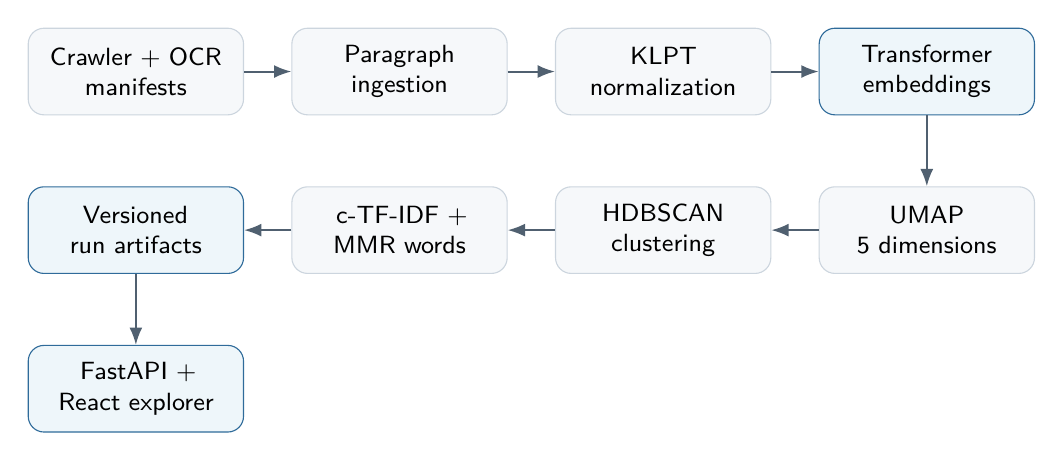
\begin{tikzpicture}[
  node distance=5mm and 6mm,
  stage/.style={rounded corners=2mm,draw=Rule,fill=Paper,minimum height=11mm,
    text width=25mm,align=center,font=\sffamily\small},
  strong/.style={stage,draw=Blue,fill=Sky!45},
  arr/.style={-{Latex[length=2.2mm]},line width=.7pt,draw=Slate}
]
\node[stage] (collect) {Crawler + OCR\\manifests};
\node[stage,right=of collect] (ingest) {Paragraph\\ingestion};
\node[stage,right=of ingest] (norm) {KLPT\\normalization};
\node[strong,right=of norm] (embed) {Transformer\\embeddings};
\node[stage,below=9mm of embed] (umap) {UMAP\\5 dimensions};
\node[stage,left=of umap] (hdb) {HDBSCAN\\clustering};
\node[stage,left=of hdb] (ctfidf) {c-TF-IDF +\\MMR words};
\node[strong,left=of ctfidf] (art) {Versioned\\run artifacts};
\node[strong,below=9mm of art] (ui) {FastAPI +\\React explorer};
\draw[arr] (collect)--(ingest);
\draw[arr] (ingest)--(norm);
\draw[arr] (norm)--(embed);
\draw[arr] (embed)--(umap);
\draw[arr] (umap)--(hdb);
\draw[arr] (hdb)--(ctfidf);
\draw[arr] (ctfidf)--(art);
\draw[arr] (art)--(ui);
\end{tikzpicture}
\caption{As-built corpus-to-interface pipeline. Fitting is performed once; ordinary exploration reads saved artifacts.}
\label{fig:pipeline}
\end{figure}

Each embedding adapter normalizes vectors to unit length and caches the complete
matrix by a content-derived key. OpenAI requests are token-aware, chunk long
documents, and use rate-limit-aware retries. NVIDIA requests use batches of 64,
up to eight concurrent workers, server-side truncation at the end, and
exponential retry for rate or server errors. UMAP reduces embeddings to five
dimensions for HDBSCAN and separately to two dimensions for display.
HDBSCAN discovers dense regions; BERTopic then reassigns eligible outliers by
c-TF-IDF similarity, extracts ten words per topic, constructs a binary topic
hierarchy, and optionally generates readable labels. Normalized pointwise
mutual information (NPMI), a coherence score based on how often a topic's top
words occur together, is computed from topic-word co-occurrence. All outputs
are written to an isolated
\sourcecode{artifacts/<source>__<model>/} directory.

\subsubsection{Tuning and reproducibility}

The production experiment is transductive and unsupervised: UMAP and HDBSCAN
are fitted on the corpus that users explore. Evaluation therefore relies on
fixed-corpus reproducibility rather than a supervised data split.
Reproducibility comes from a fixed sample, seed 42, explicit provider
identifiers, a content-keyed embedding cache, saved hyperparameters, and a
complete \sourcecode{meta.json} manifest for every run. The tuning script can
sweep HDBSCAN's minimum cluster size while reporting topic count, outlier rate,
NPMI, topic diversity, plus normalized mutual information when labels exist.

After clustering, topic naming is a separate, auditable enrichment step.
Representative keywords and passages are sent to a configured chat model,
while raw c-TF-IDF labels remain available if generation fails. FastAPI exposes
saved runs through typed endpoints, and a single in-process worker serializes
new fitting jobs to prevent competing memory-intensive pipelines. Thus model
development, inference, labeling, and presentation remain separable and can be
re-run or replaced independently.

\subsection{Hyperparameters}

Table~\ref{tab:hyperparameters} collects the key hyperparameters actually used at
each stage of the pipeline, from seeded sampling and the two UMAP projections
through HDBSCAN clustering and c-TF-IDF topic representation, to the NVIDIA
embedding adapter. Values are read directly from the deployed run manifests
and implementation rather than restated from defaults.

\begin{table}[htbp]
\centering
\caption{Key pipeline hyperparameters implemented in the repository.}
\label{tab:hyperparameters}
\small
\rowcolors{2}{RowShade}{white}
\begin{tabularx}{\linewidth}{@{}p{31mm}p{43mm}Y@{}}
\rowcolor{Navy}\thc{Stage} & \thc{Parameter} & \thc{Value}\\
Sampling & Random seed; documents & 42; 100,000\\
UMAP (clustering) & Neighbors; components; minimum distance; metric & 15; 5; 0.0; cosine\\
HDBSCAN & Minimum cluster size; minimum samples; metric & 250; 10; Euclidean\\
Topic representation & c-TF-IDF; n-grams; topic words; MMR diversity & reduced frequent words; unigrams; 10; 0.3\\
Map projection & Components; minimum distance; metric & 2; 0.1; cosine\\
NVIDIA adapter & Batch; workers; retries; truncation & 64; 8; 6; end\\
\end{tabularx}
\end{table}

% --------------------------------------------------------------------------
\clearpage
\section{Results and Evaluation}

\subsection{Production comparison}

The comparison is controlled at the corpus level: both providers received the
same sampled documents and downstream BERTopic configuration. Table
\ref{tab:results} reports the persisted measurements. NVIDIA achieved higher
topic coherence as measured by NPMI, fewer outliers, and a 10.8$\times$ shorter
end-to-end refit. OpenAI discovered six more topics, which may expose finer
distinctions but also produced more unclustered documents. Because fit time
includes cache state, provider calls, UMAP, clustering, labeling, and artifact
writing, it is an operational benchmark rather than a pure
embedding-throughput test.

\begin{table}[htbp]
\centering
\caption{Results on the identical 100,000-document deployed sample.}
\label{tab:results}
\small
\rowcolors{2}{RowShade}{white}
\begin{tabularx}{\linewidth}{@{}Yrrrrr@{}}
\rowcolor{Navy}\thc{Embedding run} & \thc{Topics} & \thc{Outliers} & \thc{Coverage} & \thc{NPMI} & \thc{Fit time (s)}\\
NVIDIA Nemotron-3-Embed-1B & 32 & 552 & 99.448\% & \textbf{0.04915} & \textbf{337.4}\\
OpenAI text-embedding-3-small & 38 & 868 & 99.132\% & 0.03742 & 3{,}628.7\\
\end{tabularx}
\end{table}

\subsection{Quality evidence and interpretation}

Normalized pointwise mutual information (NPMI) measures whether a topic's
highest-ranked words occur together more often than chance; positive values
indicate greater topic coherence. Both production runs are positive, and
NVIDIA's 0.04915 exceeds OpenAI's 0.03742 by about 31\% relative. Coverage is
the share of documents assigned to a topic and is excellent for both systems:
99,448 and 99,132 documents respectively were assigned. The NVIDIA structure
has a larger leading topic (about 15\%) than OpenAI (about 11\%), so its higher
coherence and speed come with somewhat coarser organization.

The interface supplied a second layer of practical evaluation. Automated
browser verification confirmed that topic counts and coverage update when the
embedding selector changes; the structure view opens representative documents;
the map renders a bounded 12,000-point sample; the document table paginates,
searches, and retains review states; and Insights reproduces the ingest
manifest. A live RAG trial asked, “What are the main themes in this corpus?”
The system retrieved eight passages and explicitly stated that the evidence
was too heterogeneous for a definitive answer before offering a cautious
language-and-culture interpretation. This is preferable to an unsupported
summary and demonstrates that the evidence-only prompt can abstain, although
one query is not a substitute for a formal retrieval benchmark.

\begin{figure}[htbp]
\centering
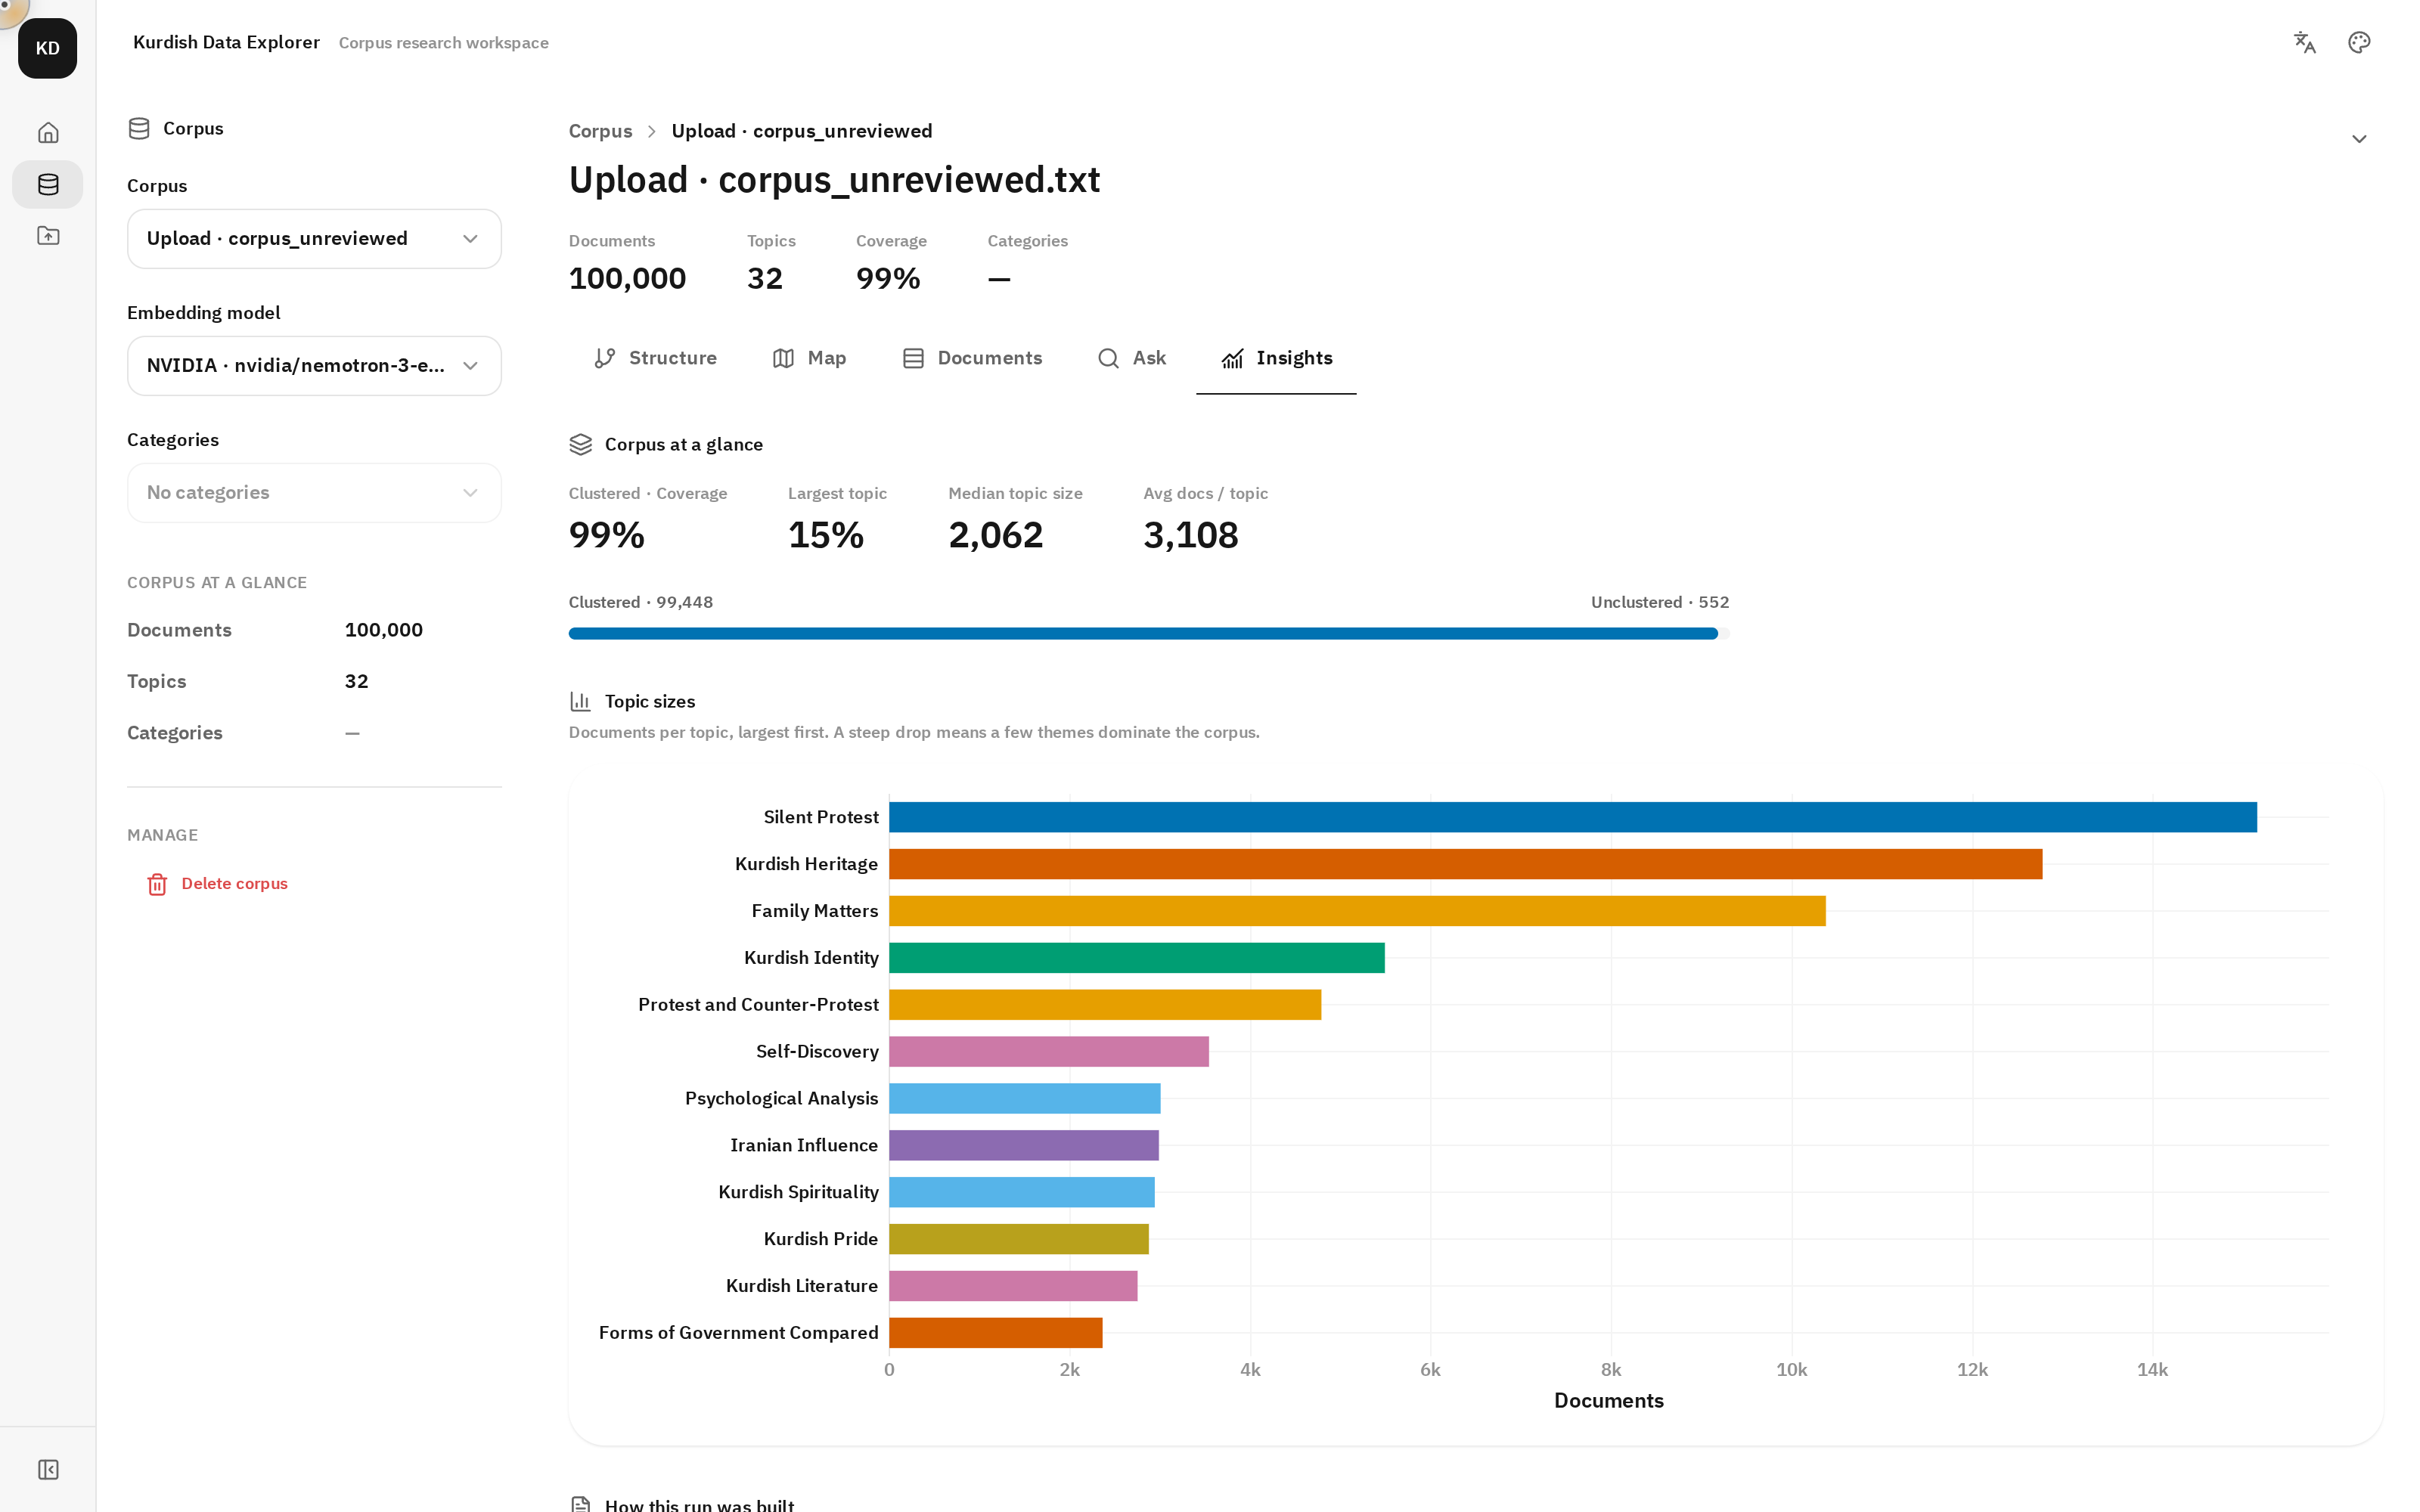
\includegraphics[width=\linewidth]{07-insights-nvidia.png}
\caption{Deployed Insights workspace for NVIDIA: 32 topics, 99\% rounded coverage, and topic-size distribution. Captured from the live application on July 24, 2026.}
\label{fig:insights-live}
\end{figure}

A confusion matrix is not applicable: the deployed data has no target classes,
and topic identifiers are arbitrary clusters rather than predicted class
labels. Substituting a confusion matrix would imply supervision that does not
exist. Appropriate evidence is therefore NPMI topic-word coherence, the share
of documents assigned rather than left as outliers, topic-size balance,
cross-model comparison, and qualitative inspection of defining terms and
representative documents.

\subsection{Observed limitations}

The evaluation reveals four practical limitations. First, corpus and OCR
outputs are explicitly unreviewed; repeated headers, dictionaries, bibliographic
pages, mixed dialects, or OCR errors can form topics. Second, automated topic
labels are generated by an LLM and may overstate what the representative
documents support. Third, two-dimensional UMAP is an exploratory projection:
distance and apparent cluster area should not be interpreted as exact semantic
geometry. Fourth, the NPMI coherence metric rewards word co-occurrence but does
not measure usefulness to a Kurdish-speaking researcher. Human topic-intrusion
and label-quality studies are still required.

% --------------------------------------------------------------------------
\section{Deployment}

\subsection{Architecture and platform}

The system is deployed at \url{\projecturl} on Fly.io. A two-stage Docker build
uses Node 20 to compile the React/Vite interface and Python 3.11 to run the
FastAPI application. One Uvicorn process serves both the static single-page
application and the \sourcecode{/api} routes on port 8080. The machine is a
\texttt{shared-cpu-2x} instance with 2 GB RAM, HTTPS enforcement, and one
always-running machine. The image includes only the approved
\sourcecode{corpus-unreviewed} OpenAI and NVIDIA artifacts and their exact
embedding caches. An mtime-keyed application cache loads one run at a time,
which avoids holding both approximately 586 MB and 782 MB embedding matrices
in limited memory.

\subsection{User interaction}

Users begin at a corpus overview and select a fitted embedding model. The
\textbf{Structure} workspace presents the topic hierarchy, terms, and
representative documents. \textbf{Map} shows a sampled 2D semantic field with
topic or density encoding. \textbf{Documents} provides text search, topic
filters, review states, nearest documents, and CSV export. \textbf{Ask}
embeds an English or Kurdish query, retrieves eight nearest passages, and asks
the configured chat model to answer only from those passages with numbered
citations. \textbf{Insights} reports topic sizes, coverage, and exact ingest
provenance. An upload workflow profiles TXT, CSV, TSV, Excel, or Parquet files
before submitting a serialized background fitting job.

\begin{figure}[htbp]
\centering
\begin{subfigure}[t]{.49\linewidth}
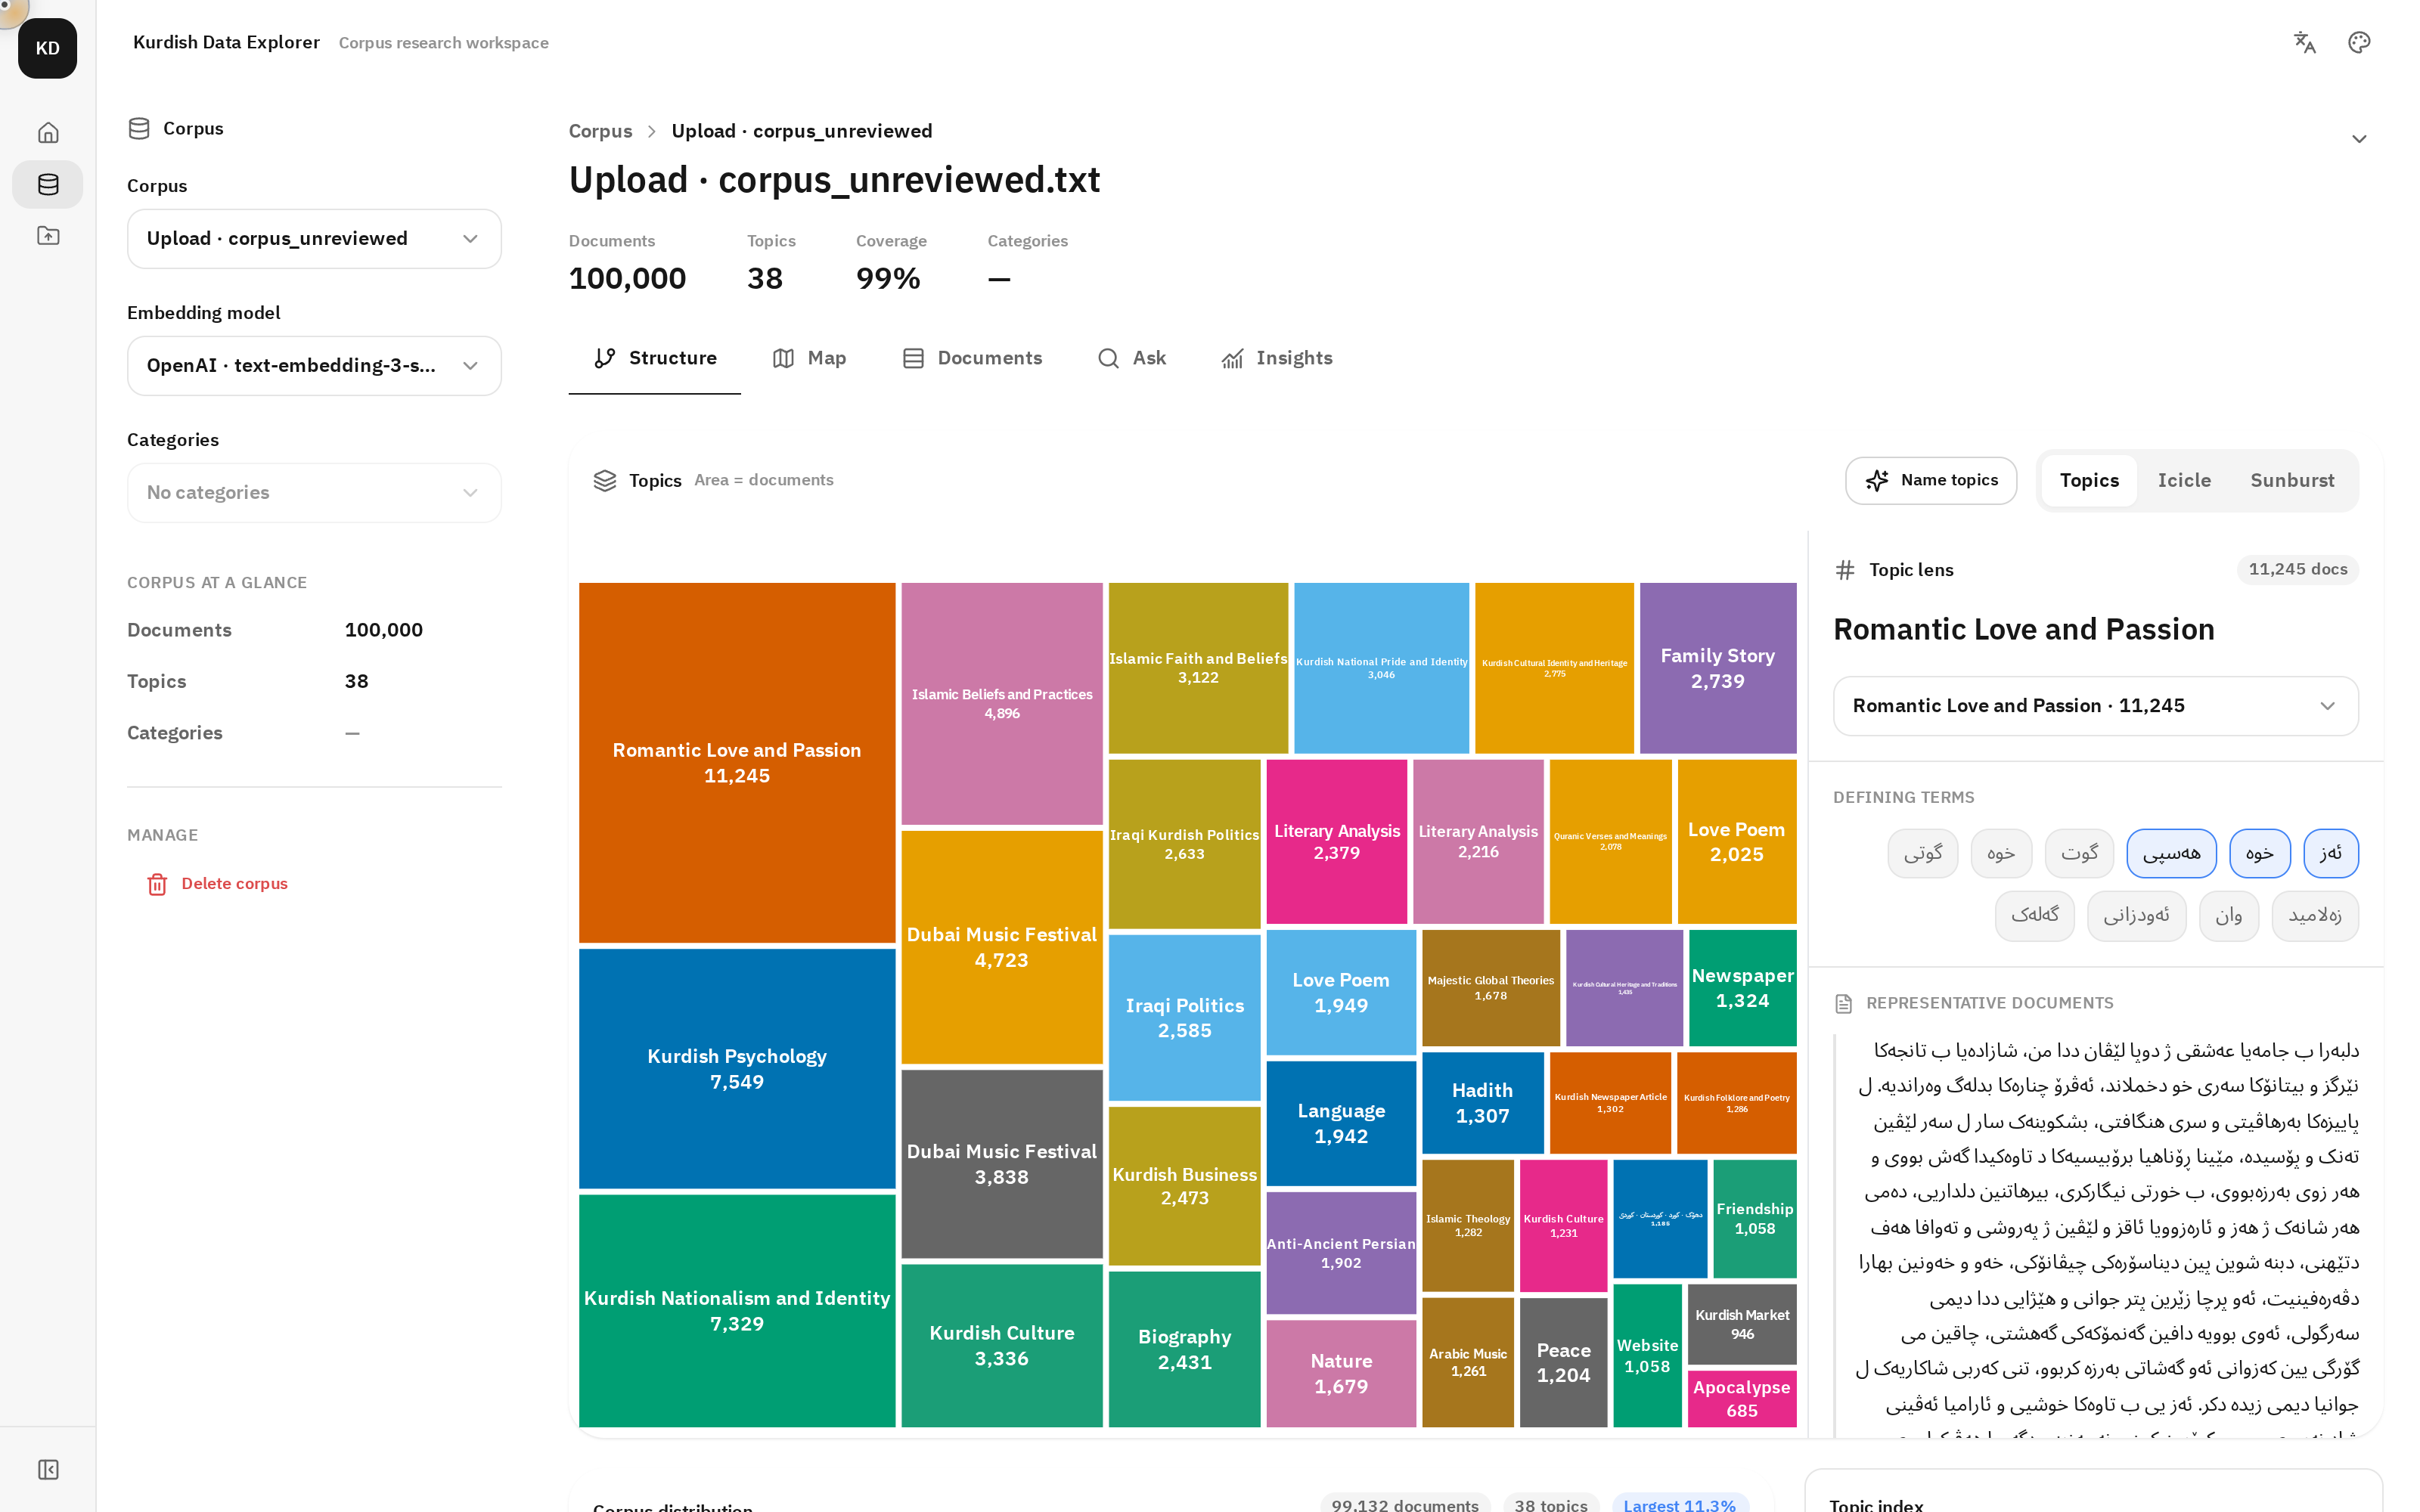
\includegraphics[width=\linewidth]{02-structure-openai.png}
\caption{Topic structure and evidence panel.}
\end{subfigure}\hfill
\begin{subfigure}[t]{.49\linewidth}
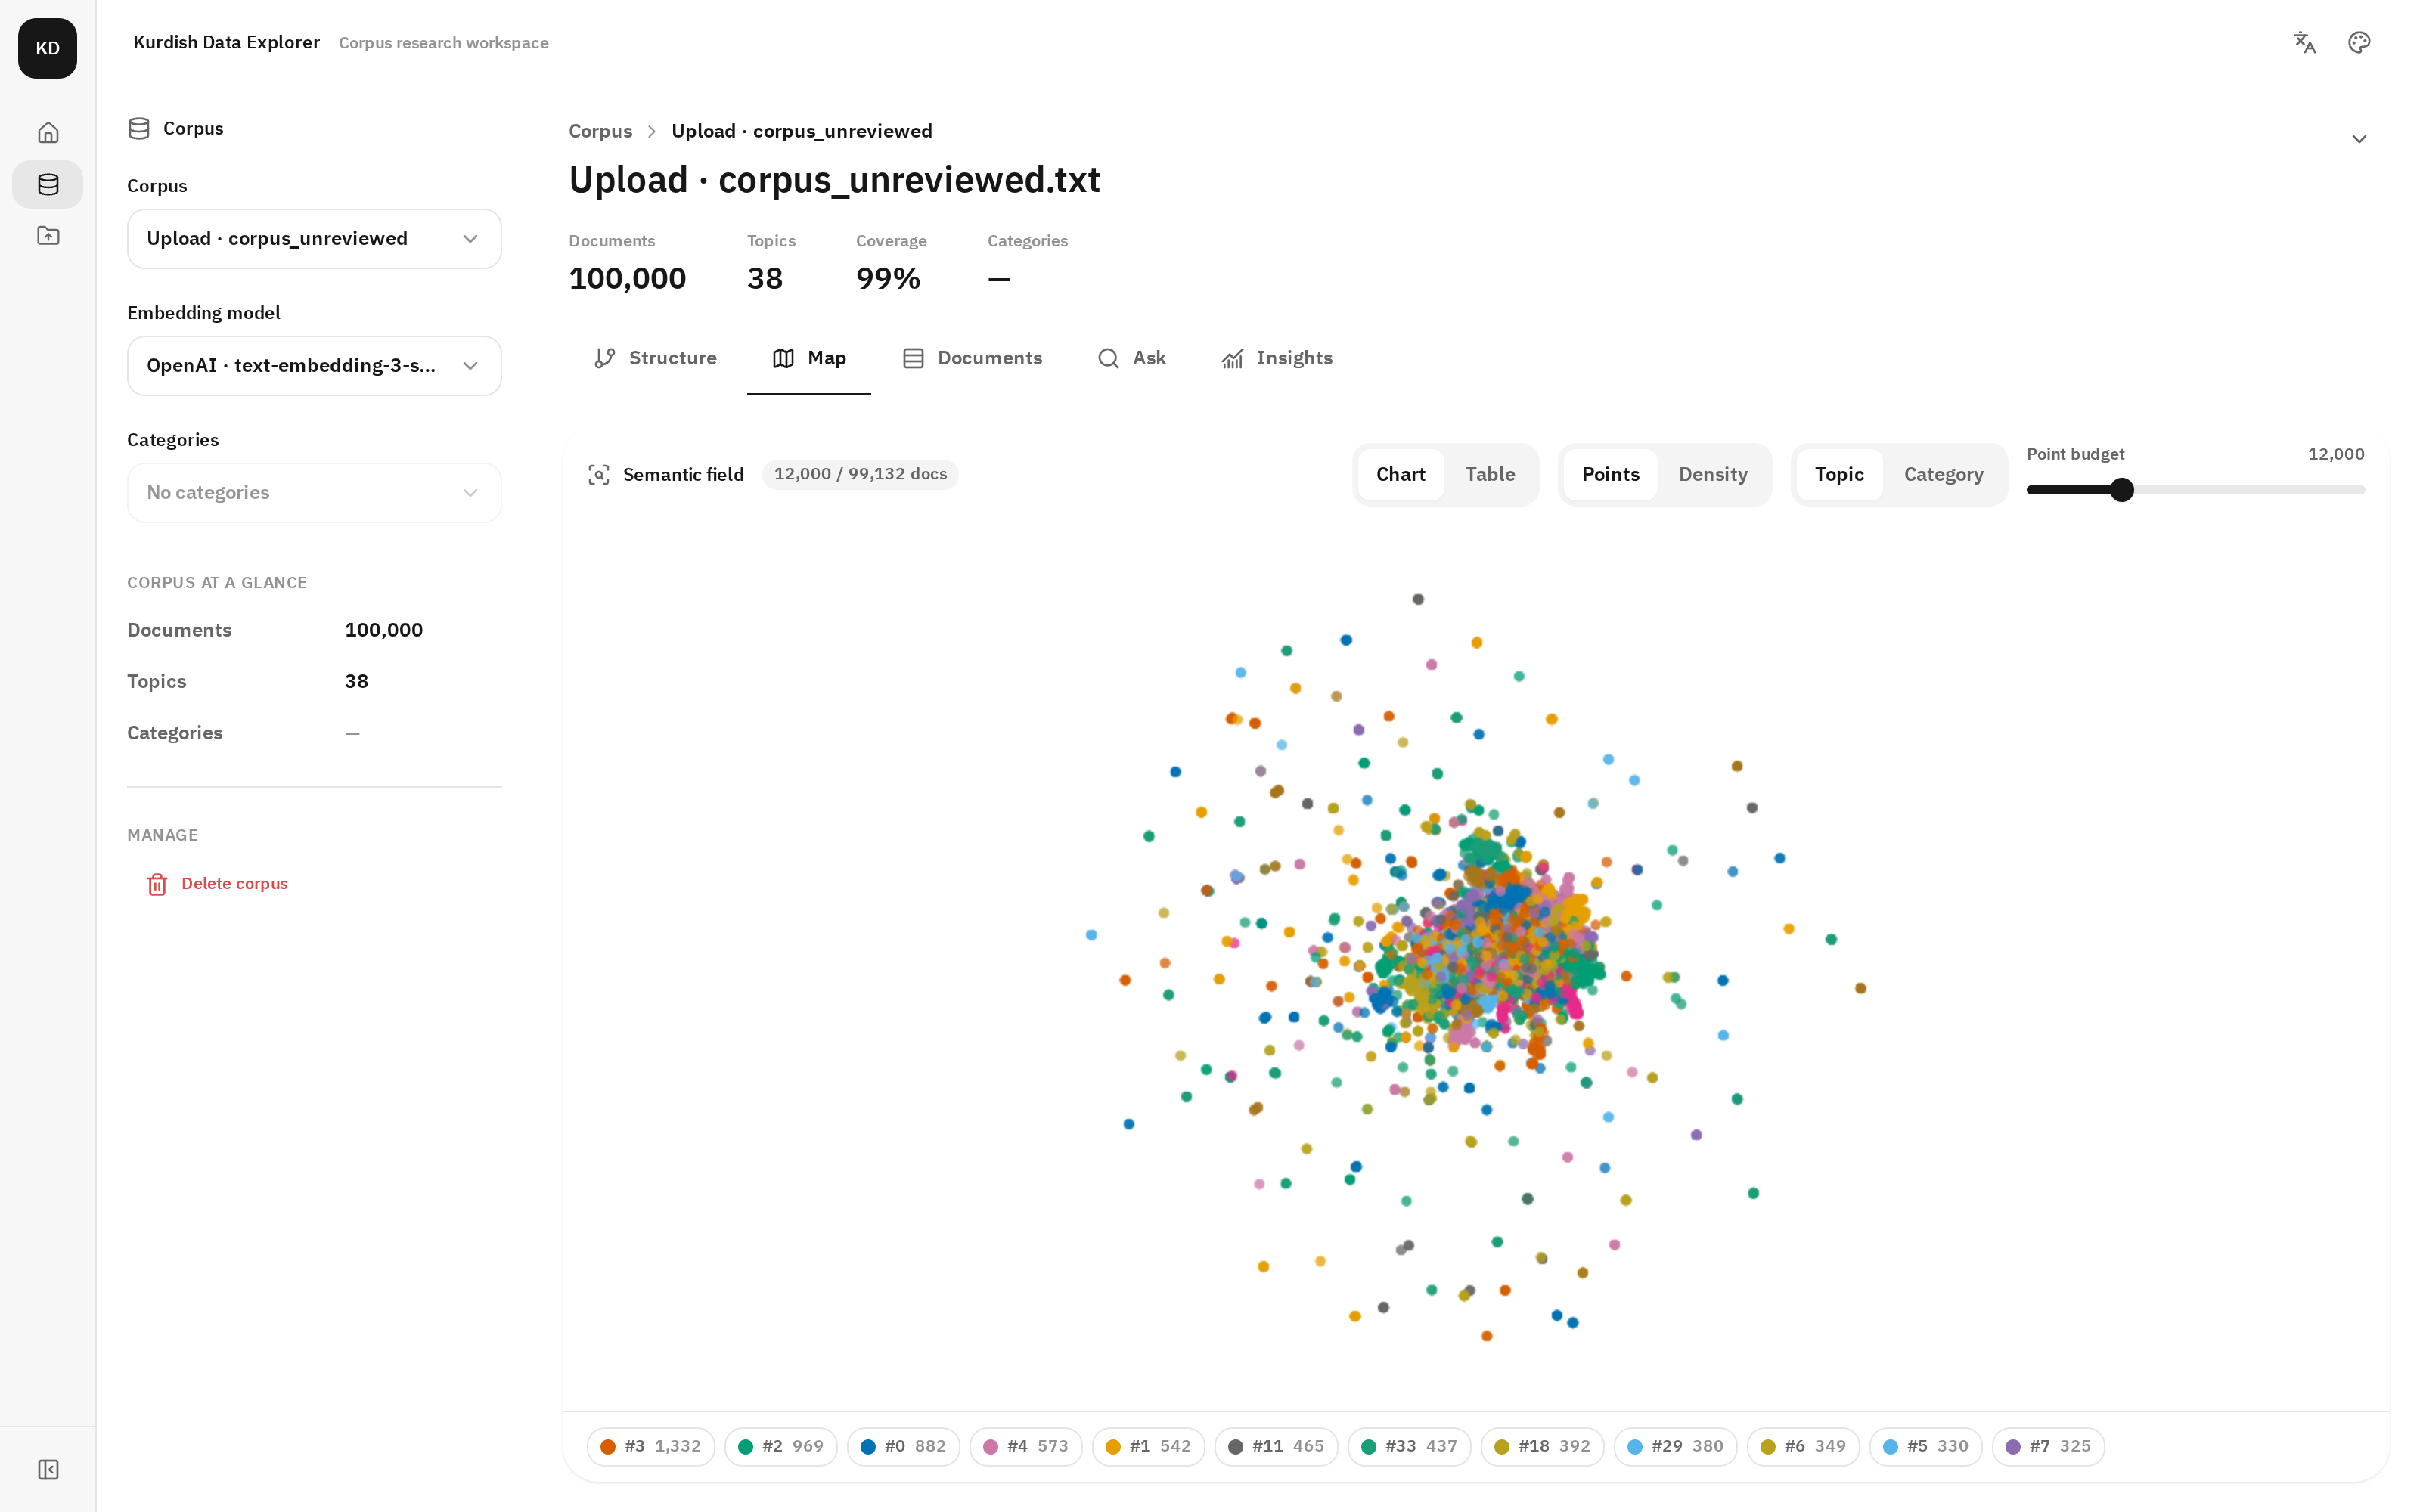
\includegraphics[width=\linewidth]{03-semantic-map-openai.png}
\caption{Interactive semantic map.}
\end{subfigure}
\caption{Two primary views in the deployed application. Full-resolution captures are provided in Appendix~\ref{app:screenshots}.}
\label{fig:deployed-views}
\end{figure}

Production verification on July 24, 2026 returned HTTP 200 and
\texttt{\{"status":"ok"\}} from \sourcecode{/api/health}; the source endpoint
reported 100,000 documents and both fitted models. Browser automation opened
the deployment, switched models, navigated every workspace, submitted a
grounded question, and recorded no console or page errors during the capture
session.

The deployment remains intentionally reproducible rather than elastic. Fitted
artifacts are baked into the image, while API keys are supplied as runtime
secrets and never committed. The health and source endpoints support release
checks; HTTPS is forced at the platform boundary. A manual prepared-checkout
deployment is currently necessary because the large corpus, embedding caches,
and vendored design-system source are excluded from a clean public clone.

% --------------------------------------------------------------------------
\section{Conclusion and Future Improvements}

Kurdish Data Explorer demonstrates a complete applied-AI workflow: source
collection with provenance, corpus preparation, transformer embedding,
unsupervised topic discovery, measurable evaluation, artifact persistence, a
usable research interface, RAG-based evidence access, and public deployment.
The fixed 100,000-document comparison makes the main result concrete. NVIDIA
offered the strongest operational trade-off in this run: higher topic-word
coherence, fewer outliers, and substantially lower fit time, while OpenAI
exposed a finer 38-topic structure. The result is not simply a model notebook;
it is an inspectable system in which users can trace topics and answers back to
text.

The next development phase should prioritize data quality over adding another
model. OCR outputs should pass document-level human review, duplicates and
boilerplate should be removed, licenses and source permissions should be
audited, and Bahdini-specific normalization should replace the current
Sorani-oriented configuration. Evaluation should add Kurdish-speaker topic
intrusion, word intrusion, label correctness, and task-completion studies.
Technically, durable job storage, approximate-nearest-neighbor search, streaming
artifact loading, provider-cost logging, and role-based review would support
larger corpora and collaborative use. Finally, a held-out, manually labelled
Bahdini evaluation set would enable normalized mutual information, which
measures agreement between discovered topics and human labels, as well as
controlled downstream retrieval tests without misrepresenting unsupervised
topics as classes.

\clearpage
\printbibliography[heading=bibintoc,title={References}]

% --------------------------------------------------------------------------
\appendix
\clearpage
\phantomsection
\addcontentsline{toc}{section}{Appendix}
\section*{Appendix}
\markboth{Appendix}{Appendix}

\refstepcounter{section}
\subsection*{Appendix~\thesection: System Architecture Diagrams}
\addcontentsline{toc}{subsection}{Appendix~\thesection: System Architecture Diagrams}
\label{app:diagrams}
\begin{figure}[htbp]
\centering
\resizebox{\linewidth}{!}{%
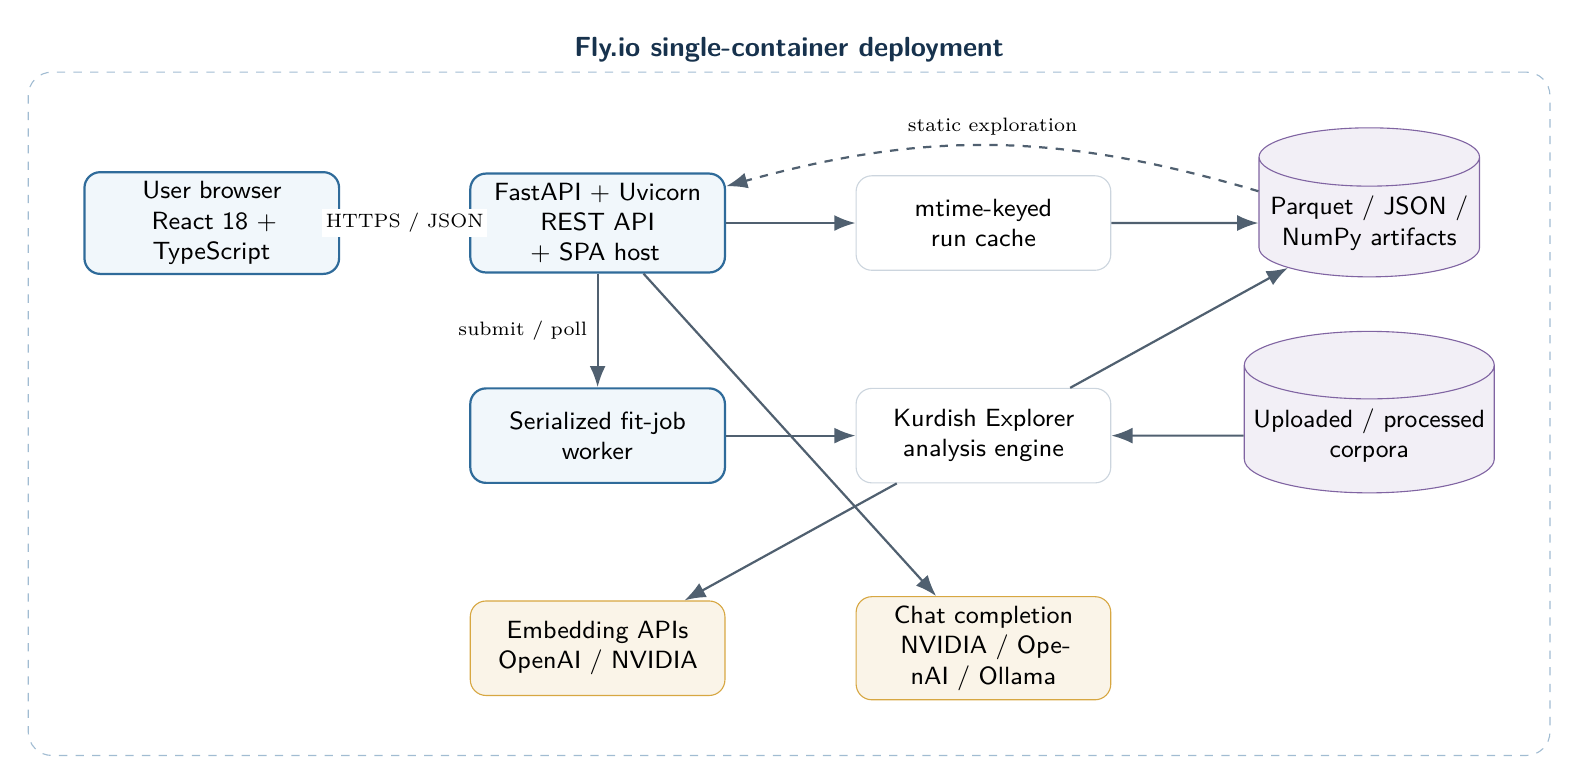
\begin{tikzpicture}[
  font=\sffamily\small,
  box/.style={rounded corners=2mm,draw=Rule,fill=white,minimum height=12mm,
    text width=30mm,align=center},
  primary/.style={box,draw=Blue,line width=.8pt,fill=Sky!38},
  data/.style={cylinder,shape border rotate=90,aspect=.27,draw=Purple,
    fill=Purple!10,minimum width=28mm,minimum height=15mm,align=center},
  ext/.style={box,draw=Gold,fill=Gold!12},
  arrow/.style={-{Latex[length=2.7mm]},line width=.8pt,draw=Slate},
  dashedarrow/.style={arrow,dashed}
]
% Explicit coordinates keep every box in its own cell; external-service
% nodes sit in the gaps between columns so nothing overlaps.
% Wide column spacing (4.9) leaves room for the edge labels so no label
% overlaps an arrow or a box.
\node[primary] (browser) at (0,0) {User browser\\React 18 + TypeScript};
\node[primary] (api) at (4.9,0) {FastAPI + Uvicorn\\REST API + SPA host};
\node[box] (cache) at (9.8,0) {mtime-keyed\\run cache};
\node[data] (artifacts) at (14.7,0) {Parquet / JSON /\\NumPy artifacts};

\node[primary] (jobs) at (4.9,-2.7) {Serialized fit-job\\worker};
\node[box] (engine) at (9.8,-2.7) {Kurdish Explorer\\analysis engine};
\node[data] (corpus) at (14.7,-2.7) {Uploaded / processed\\corpora};

\node[ext] (providers) at (4.9,-5.4) {Embedding APIs\\OpenAI / NVIDIA};
\node[ext] (chat) at (9.8,-5.4) {Chat completion\\NVIDIA / OpenAI / Ollama};

\draw[arrow] (browser) -- node[midway,fill=white,inner sep=1.4pt,font=\scriptsize]{HTTPS / JSON} (api);
\draw[arrow] (api) -- (cache);
\draw[arrow] (cache) -- (artifacts);
\draw[arrow] (api) -- node[midway,left=2pt,fill=white,inner sep=1.4pt,font=\scriptsize]{submit / poll} (jobs);
\draw[arrow] (jobs) -- (engine);
\draw[arrow] (corpus) -- (engine);
\draw[arrow] (engine) -- (artifacts);
\draw[arrow] (engine) -- (providers);
\draw[arrow] (api) -- (chat);
\draw[dashedarrow] (artifacts) to[bend right=16] node[midway,above,font=\scriptsize]{static exploration} (api);

\begin{scope}[on background layer]
\node[draw=Blue!45,dashed,rounded corners=3mm,fit=(browser)(api)(cache)(artifacts)(jobs)(engine)(corpus)(providers)(chat),
  inner sep=7mm,label={[font=\sffamily\bfseries\color{Navy}]above:Fly.io single-container deployment}] {};
\end{scope}
\end{tikzpicture}
}
\caption{Production component architecture. Expensive fitting uses a serialized worker; ordinary browsing reads immutable run artifacts through the cache.}
\label{fig:architecture}
\end{figure}

\begin{figure}[htbp]
\centering
\resizebox{.60\linewidth}{!}{%
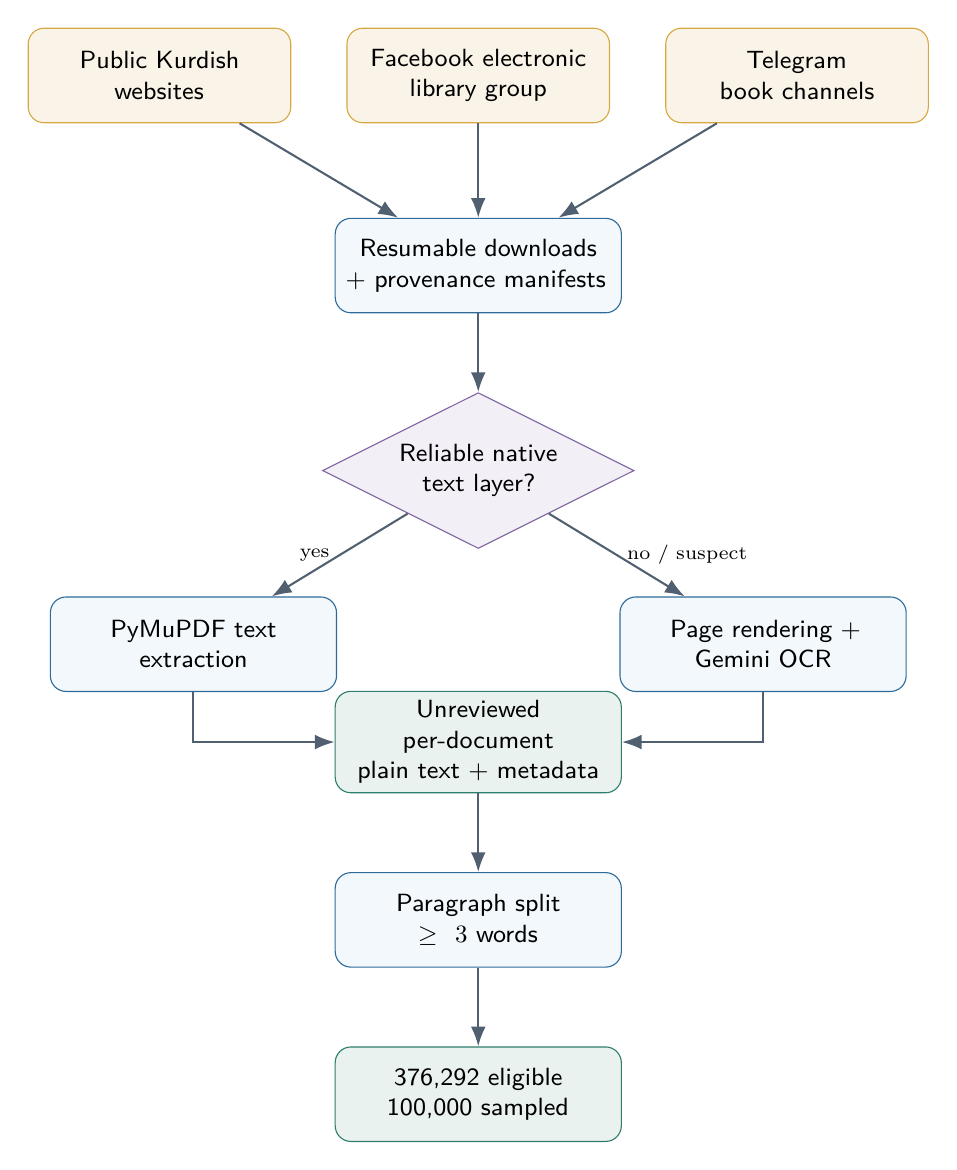
\begin{tikzpicture}[
  font=\sffamily\small,
  source/.style={rounded corners=2mm,draw=Gold,fill=Gold!12,text width=31mm,
    minimum height=12mm,align=center},
  process/.style={rounded corners=2mm,draw=Blue,fill=Sky!35,text width=34mm,
    minimum height=12mm,align=center},
  decision/.style={diamond,aspect=2.0,draw=Purple,fill=Purple!10,text width=23mm,
    align=center,inner sep=1.5pt},
  output/.style={rounded corners=2mm,draw=Green,fill=Green!10,text width=34mm,
    minimum height=12mm,align=center},
  arrow/.style={-{Latex[length=2.5mm]},line width=.75pt,draw=Slate}
]
\node[source] (web) {Public Kurdish\\websites};
\node[source,right=7mm of web] (fb) {Facebook electronic\\library group};
\node[source,right=7mm of fb] (tg) {Telegram\\book channels};

\node[process,below=12mm of fb] (manifest) {Resumable downloads\\+ provenance manifests};
\node[decision,below=10mm of manifest] (extract) {Reliable native\\text layer?};
\node[process,below left=11mm and 8mm of extract] (native) {PyMuPDF text\\extraction};
\node[process,below right=11mm and 8mm of extract] (ocr) {Page rendering +\\Gemini OCR};
\node[output,below=18mm of extract] (unreviewed) {Unreviewed per-document\\plain text + metadata};
\node[process,below=10mm of unreviewed] (compile) {Paragraph split\\$\geq 3$ words};
\node[output,below=10mm of compile] (sample) {376,292 eligible\\100,000 sampled};

\draw[arrow] (web) -- (manifest);
\draw[arrow] (fb) -- (manifest);
\draw[arrow] (tg) -- (manifest);
\draw[arrow] (manifest) -- (extract);
\draw[arrow] (extract) -- node[left,font=\scriptsize]{yes} (native);
\draw[arrow] (extract) -- node[right,font=\scriptsize]{no / suspect} (ocr);
\draw[arrow] (native) |- (unreviewed);
\draw[arrow] (ocr) |- (unreviewed);
\draw[arrow] (unreviewed) -- (compile);
\draw[arrow] (compile) -- (sample);
\end{tikzpicture}
}
\caption{Verified corpus provenance from Bahdini Crawler to the deployed analytical sample. “Unreviewed” is retained as an explicit quality state.}
\label{fig:provenance}
\end{figure}

\begin{figure}[htbp]
\centering
\resizebox{.80\linewidth}{!}{%
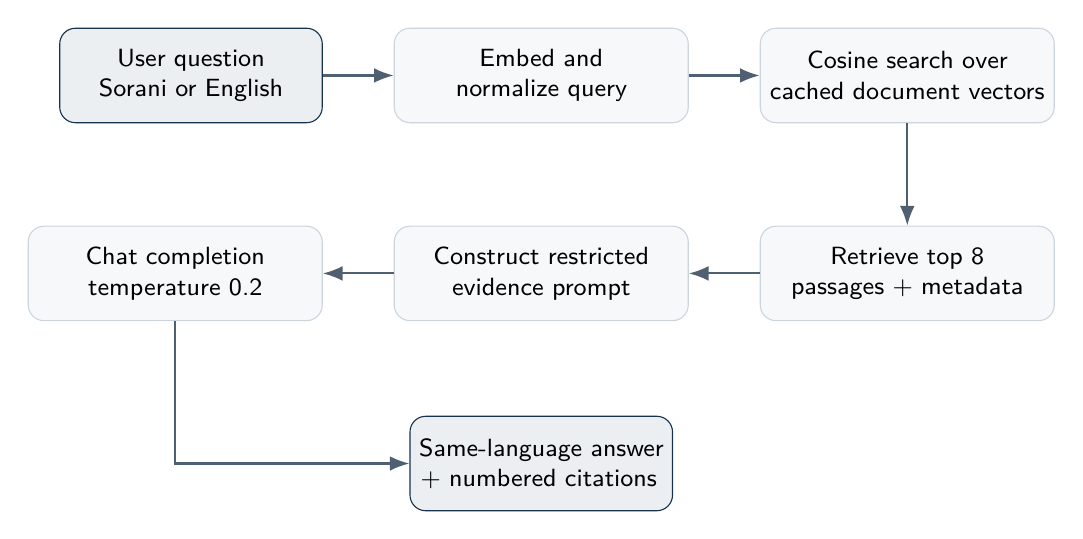
\begin{tikzpicture}[
  font=\sffamily\small,
  actor/.style={rounded corners=2mm,draw=Navy,fill=Navy!8,text width=31mm,
    minimum height=12mm,align=center},
  procstep/.style={rounded corners=2mm,draw=Rule,fill=Paper,text width=35mm,
    minimum height=12mm,align=center},
  arrow/.style={-{Latex[length=2.5mm]},line width=.75pt,draw=Slate}
]
\node[actor] (user) {User question\\Sorani or English};
\node[procstep,right=9mm of user] (qembed) {Embed and\\normalize query};
\node[procstep,right=9mm of qembed] (search) {Cosine search over\\cached document vectors};
\node[procstep,below=13mm of search] (topk) {Retrieve top 8\\passages + metadata};
\node[procstep,left=9mm of topk] (prompt) {Construct restricted\\evidence prompt};
\node[procstep,left=9mm of prompt] (llm) {Chat completion\\temperature 0.2};
\node[actor,below=12mm of prompt] (answer) {Same-language answer\\+ numbered citations};
\draw[arrow] (user)--(qembed);
\draw[arrow] (qembed)--(search);
\draw[arrow] (search)--(topk);
\draw[arrow] (topk)--(prompt);
\draw[arrow] (prompt)--(llm);
\draw[arrow] (llm) |- (answer);
\end{tikzpicture}
}
\caption{Grounded question-answering flow. The instruction requires the model to use only retrieved passages and to state when evidence is insufficient.}
\label{fig:rag}
\end{figure}

% --------------------------------------------------------------------------
\clearpage
\refstepcounter{section}
\subsection*{Appendix~\thesection: Live System Screenshots}
\addcontentsline{toc}{subsection}{Appendix~\thesection: Live System Screenshots}
\label{app:screenshots}
\begin{figure}[htbp]
\centering
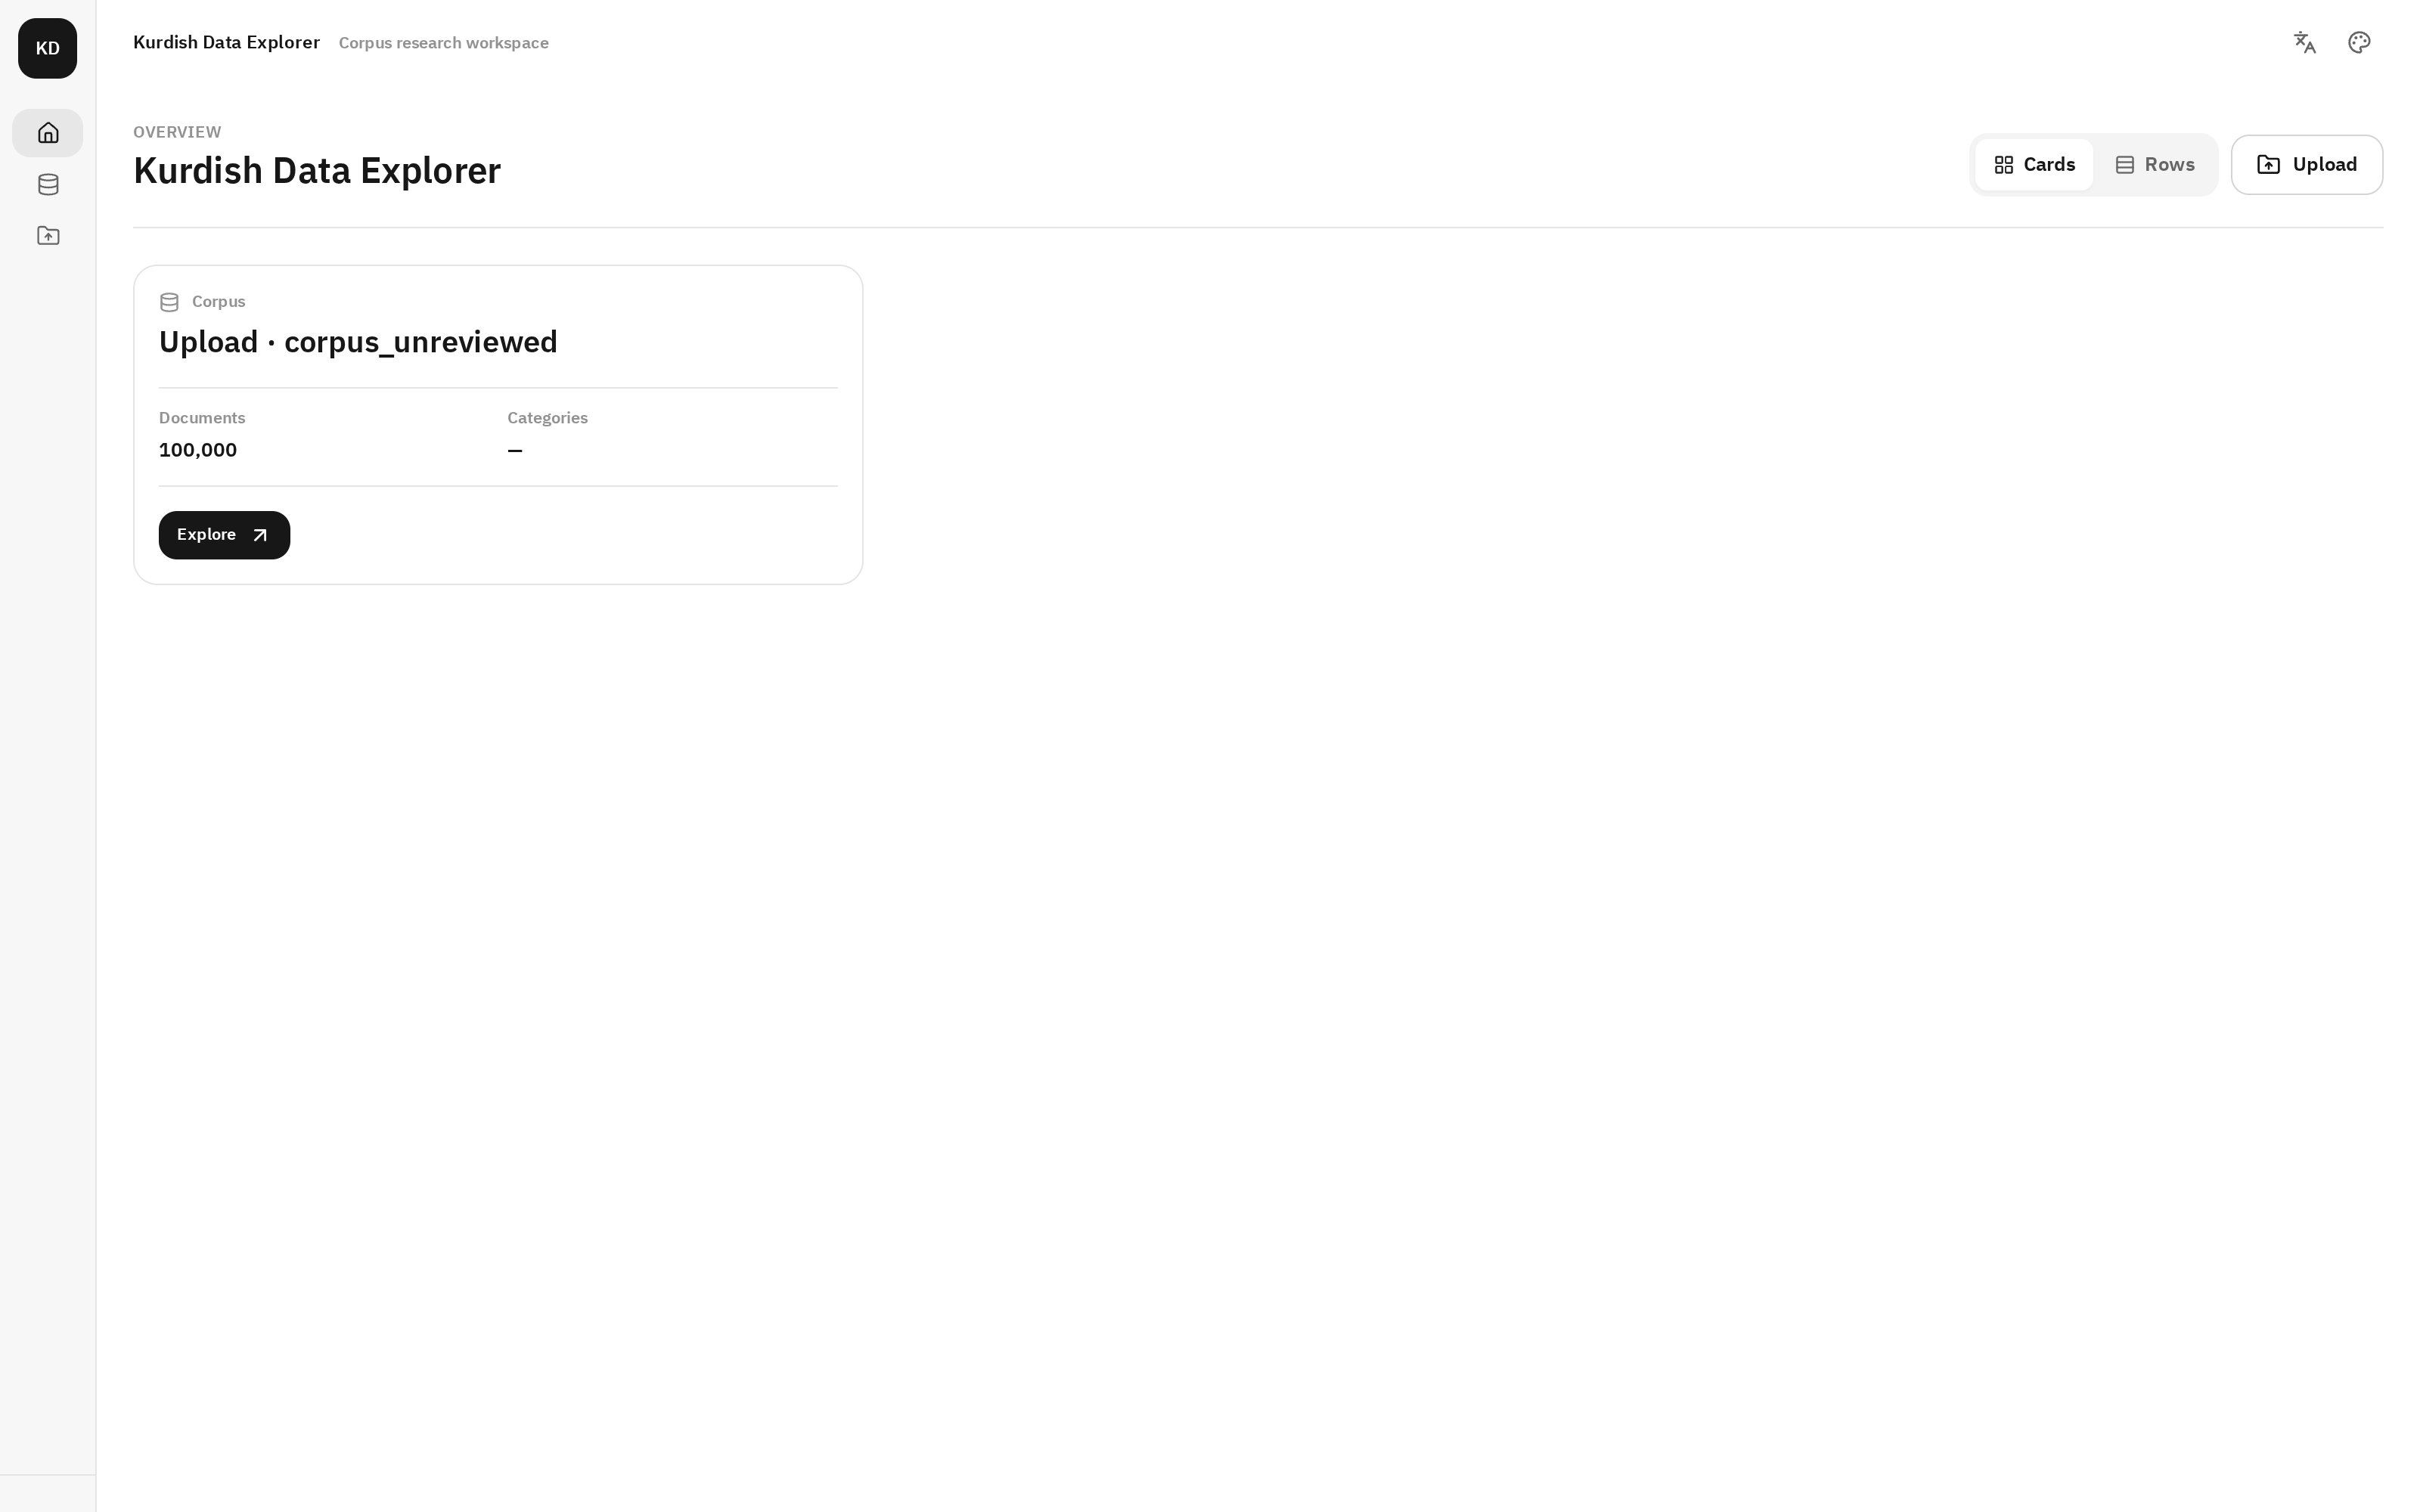
\includegraphics[width=\linewidth]{01-overview.png}
\caption{Corpus overview: the controlled deployment exposes one 100,000-document source.}
\end{figure}

\begin{figure}[htbp]
\centering
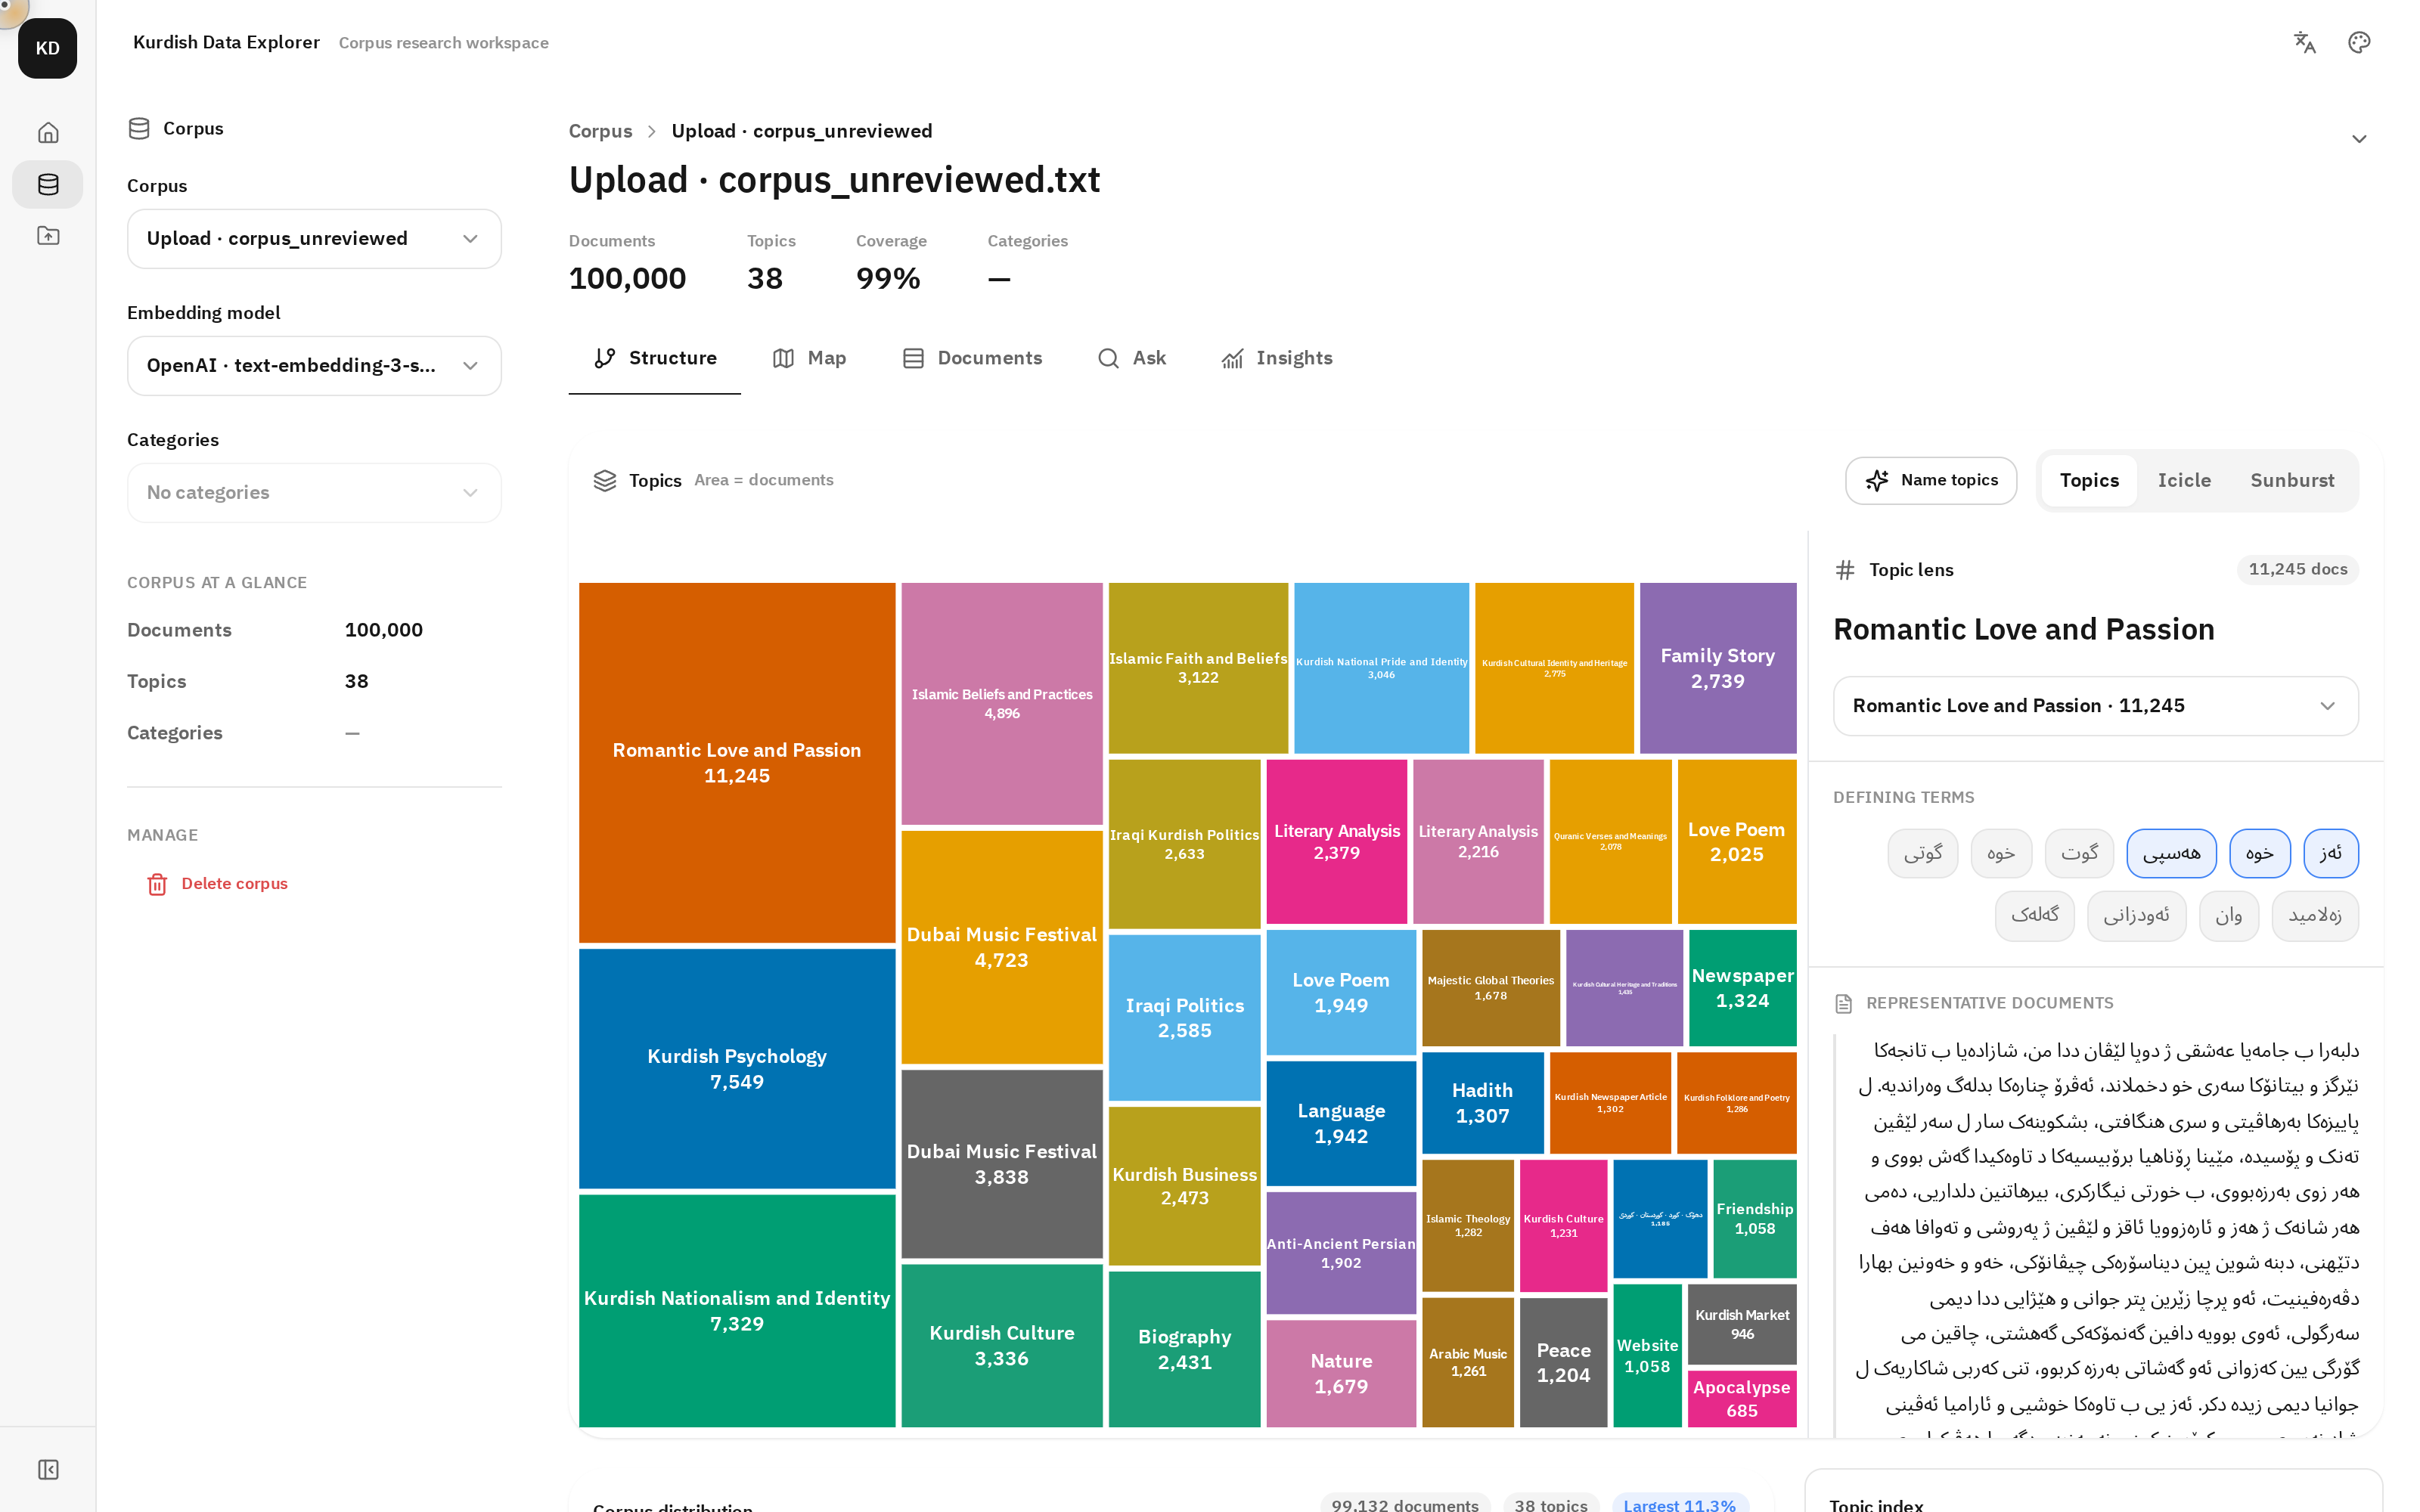
\includegraphics[width=\linewidth]{02-structure-openai.png}
\caption{Structure workspace: topic treemap, defining terms, and representative Kurdish documents.}
\end{figure}

\begin{figure}[htbp]
\centering
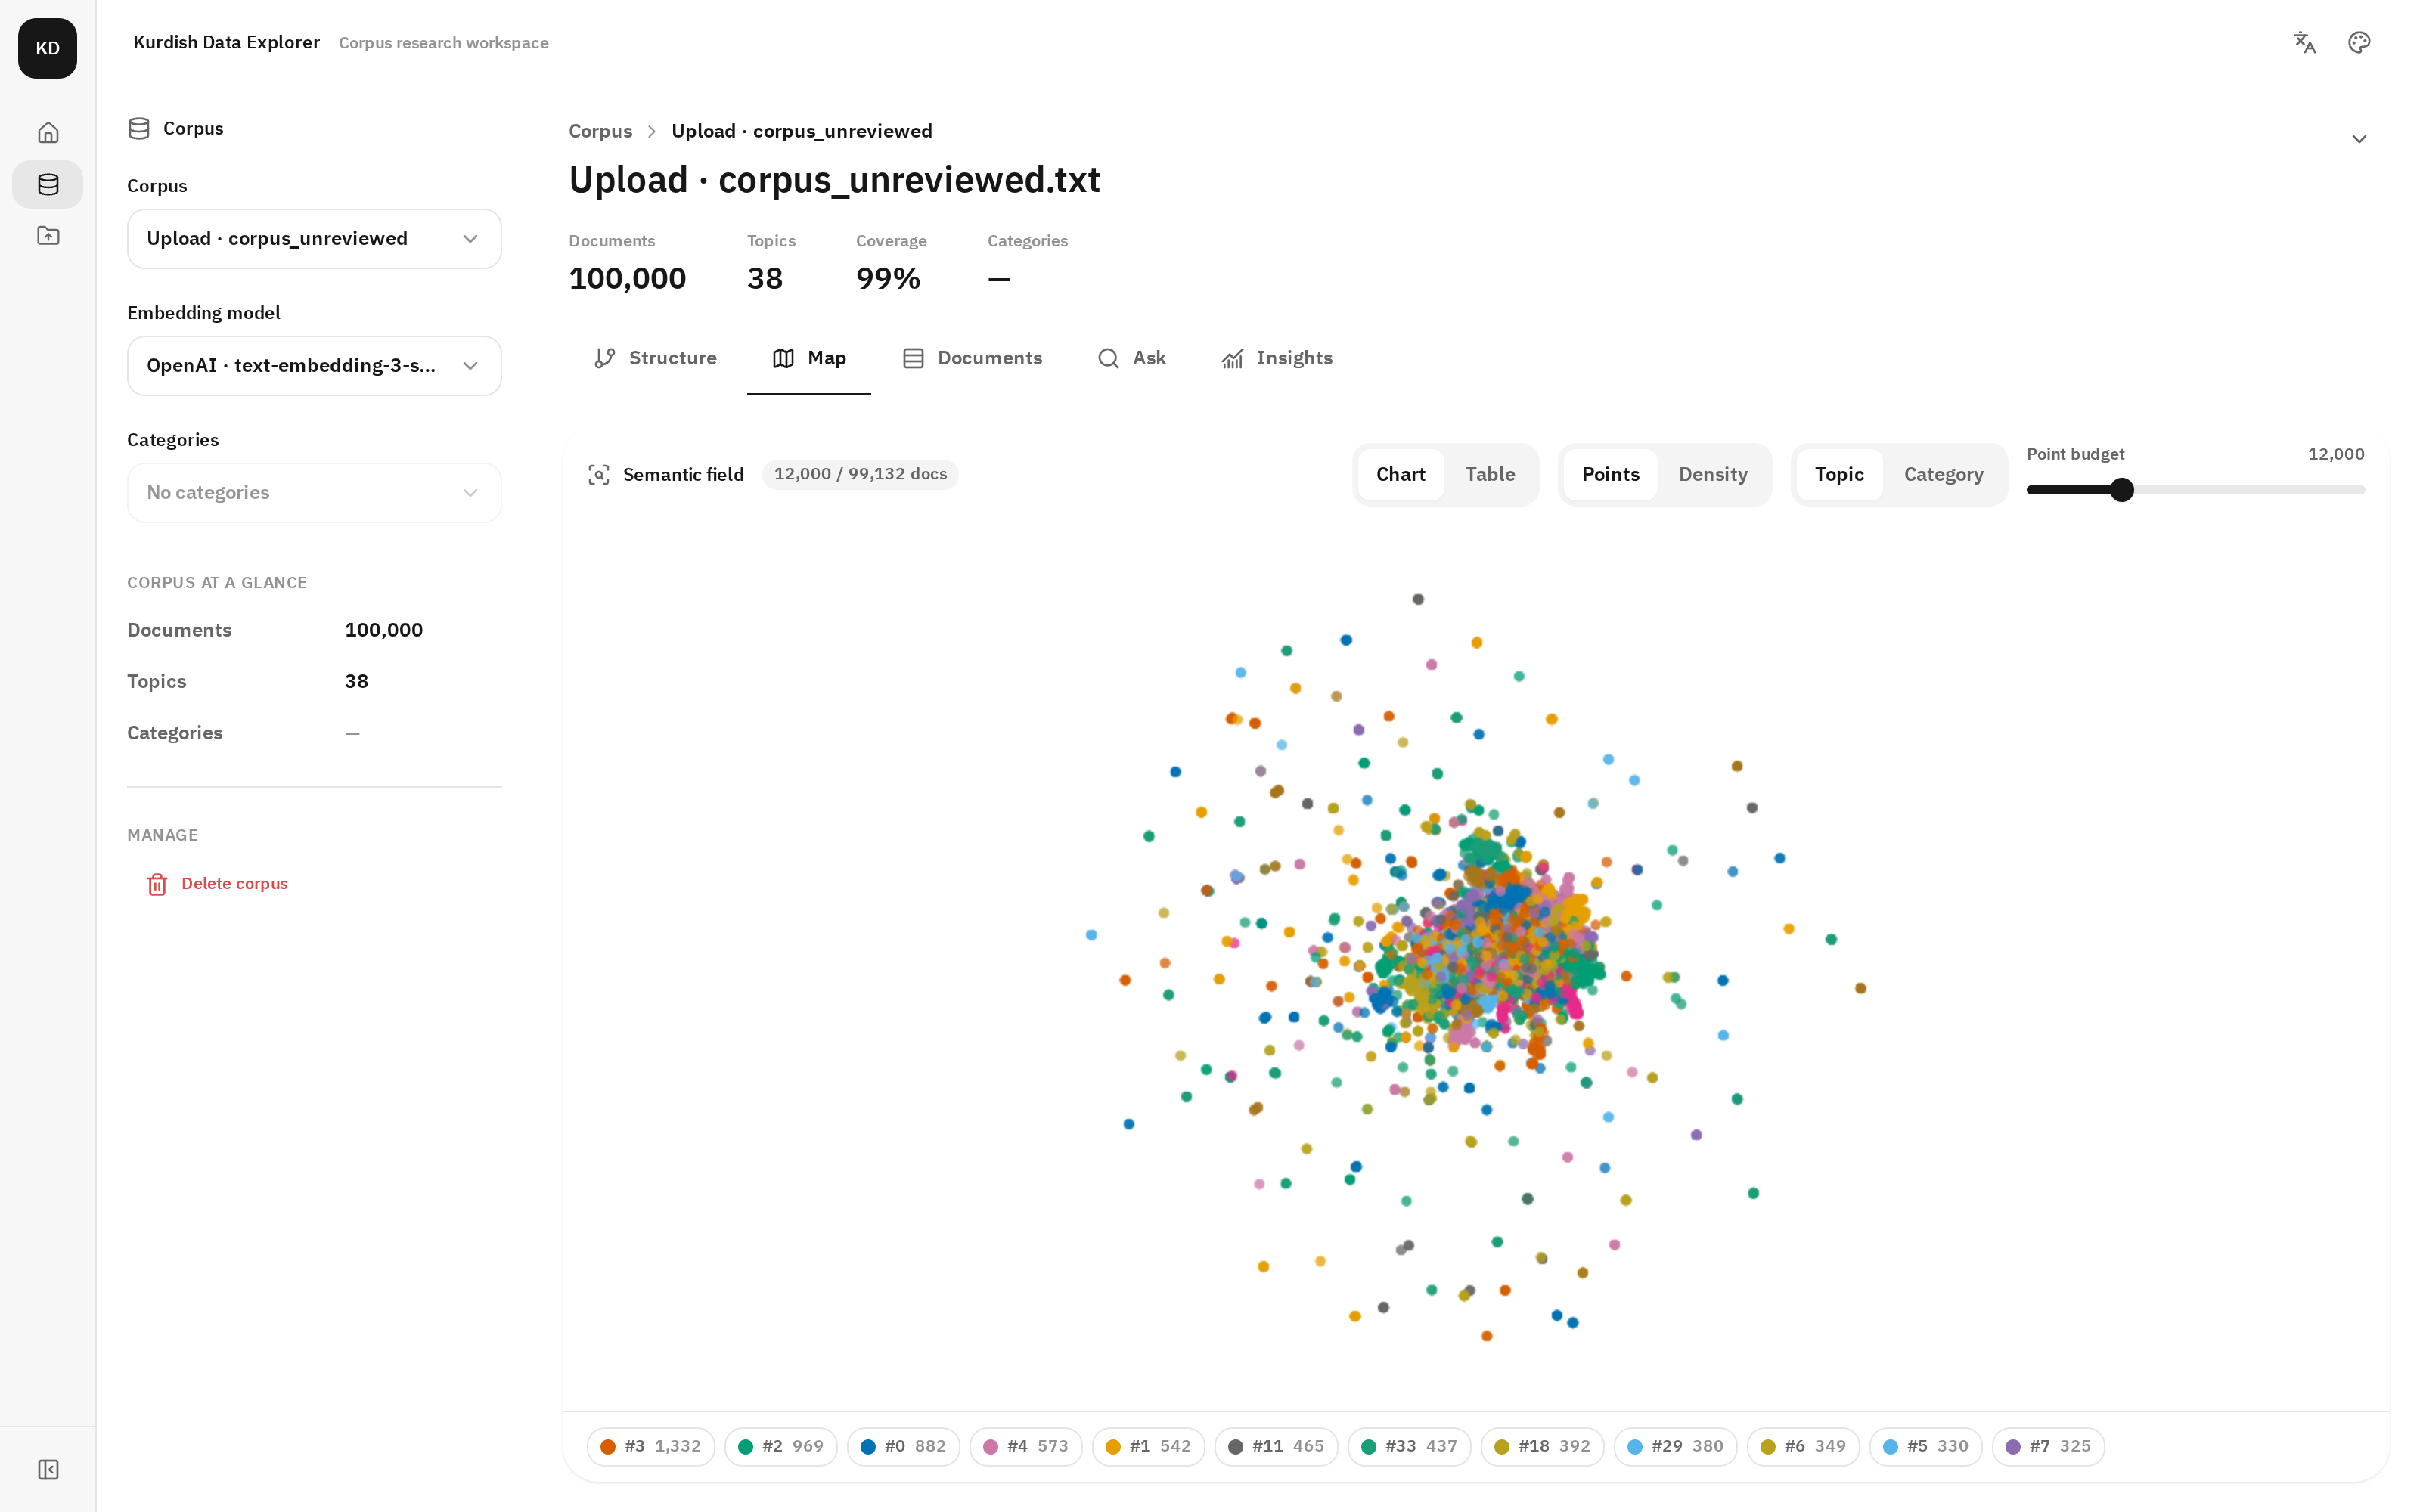
\includegraphics[width=\linewidth]{03-semantic-map-openai.png}
\caption{Map workspace: 12,000 displayed points sampled from 99,132 clustered OpenAI documents.}
\end{figure}

\begin{figure}[htbp]
\centering
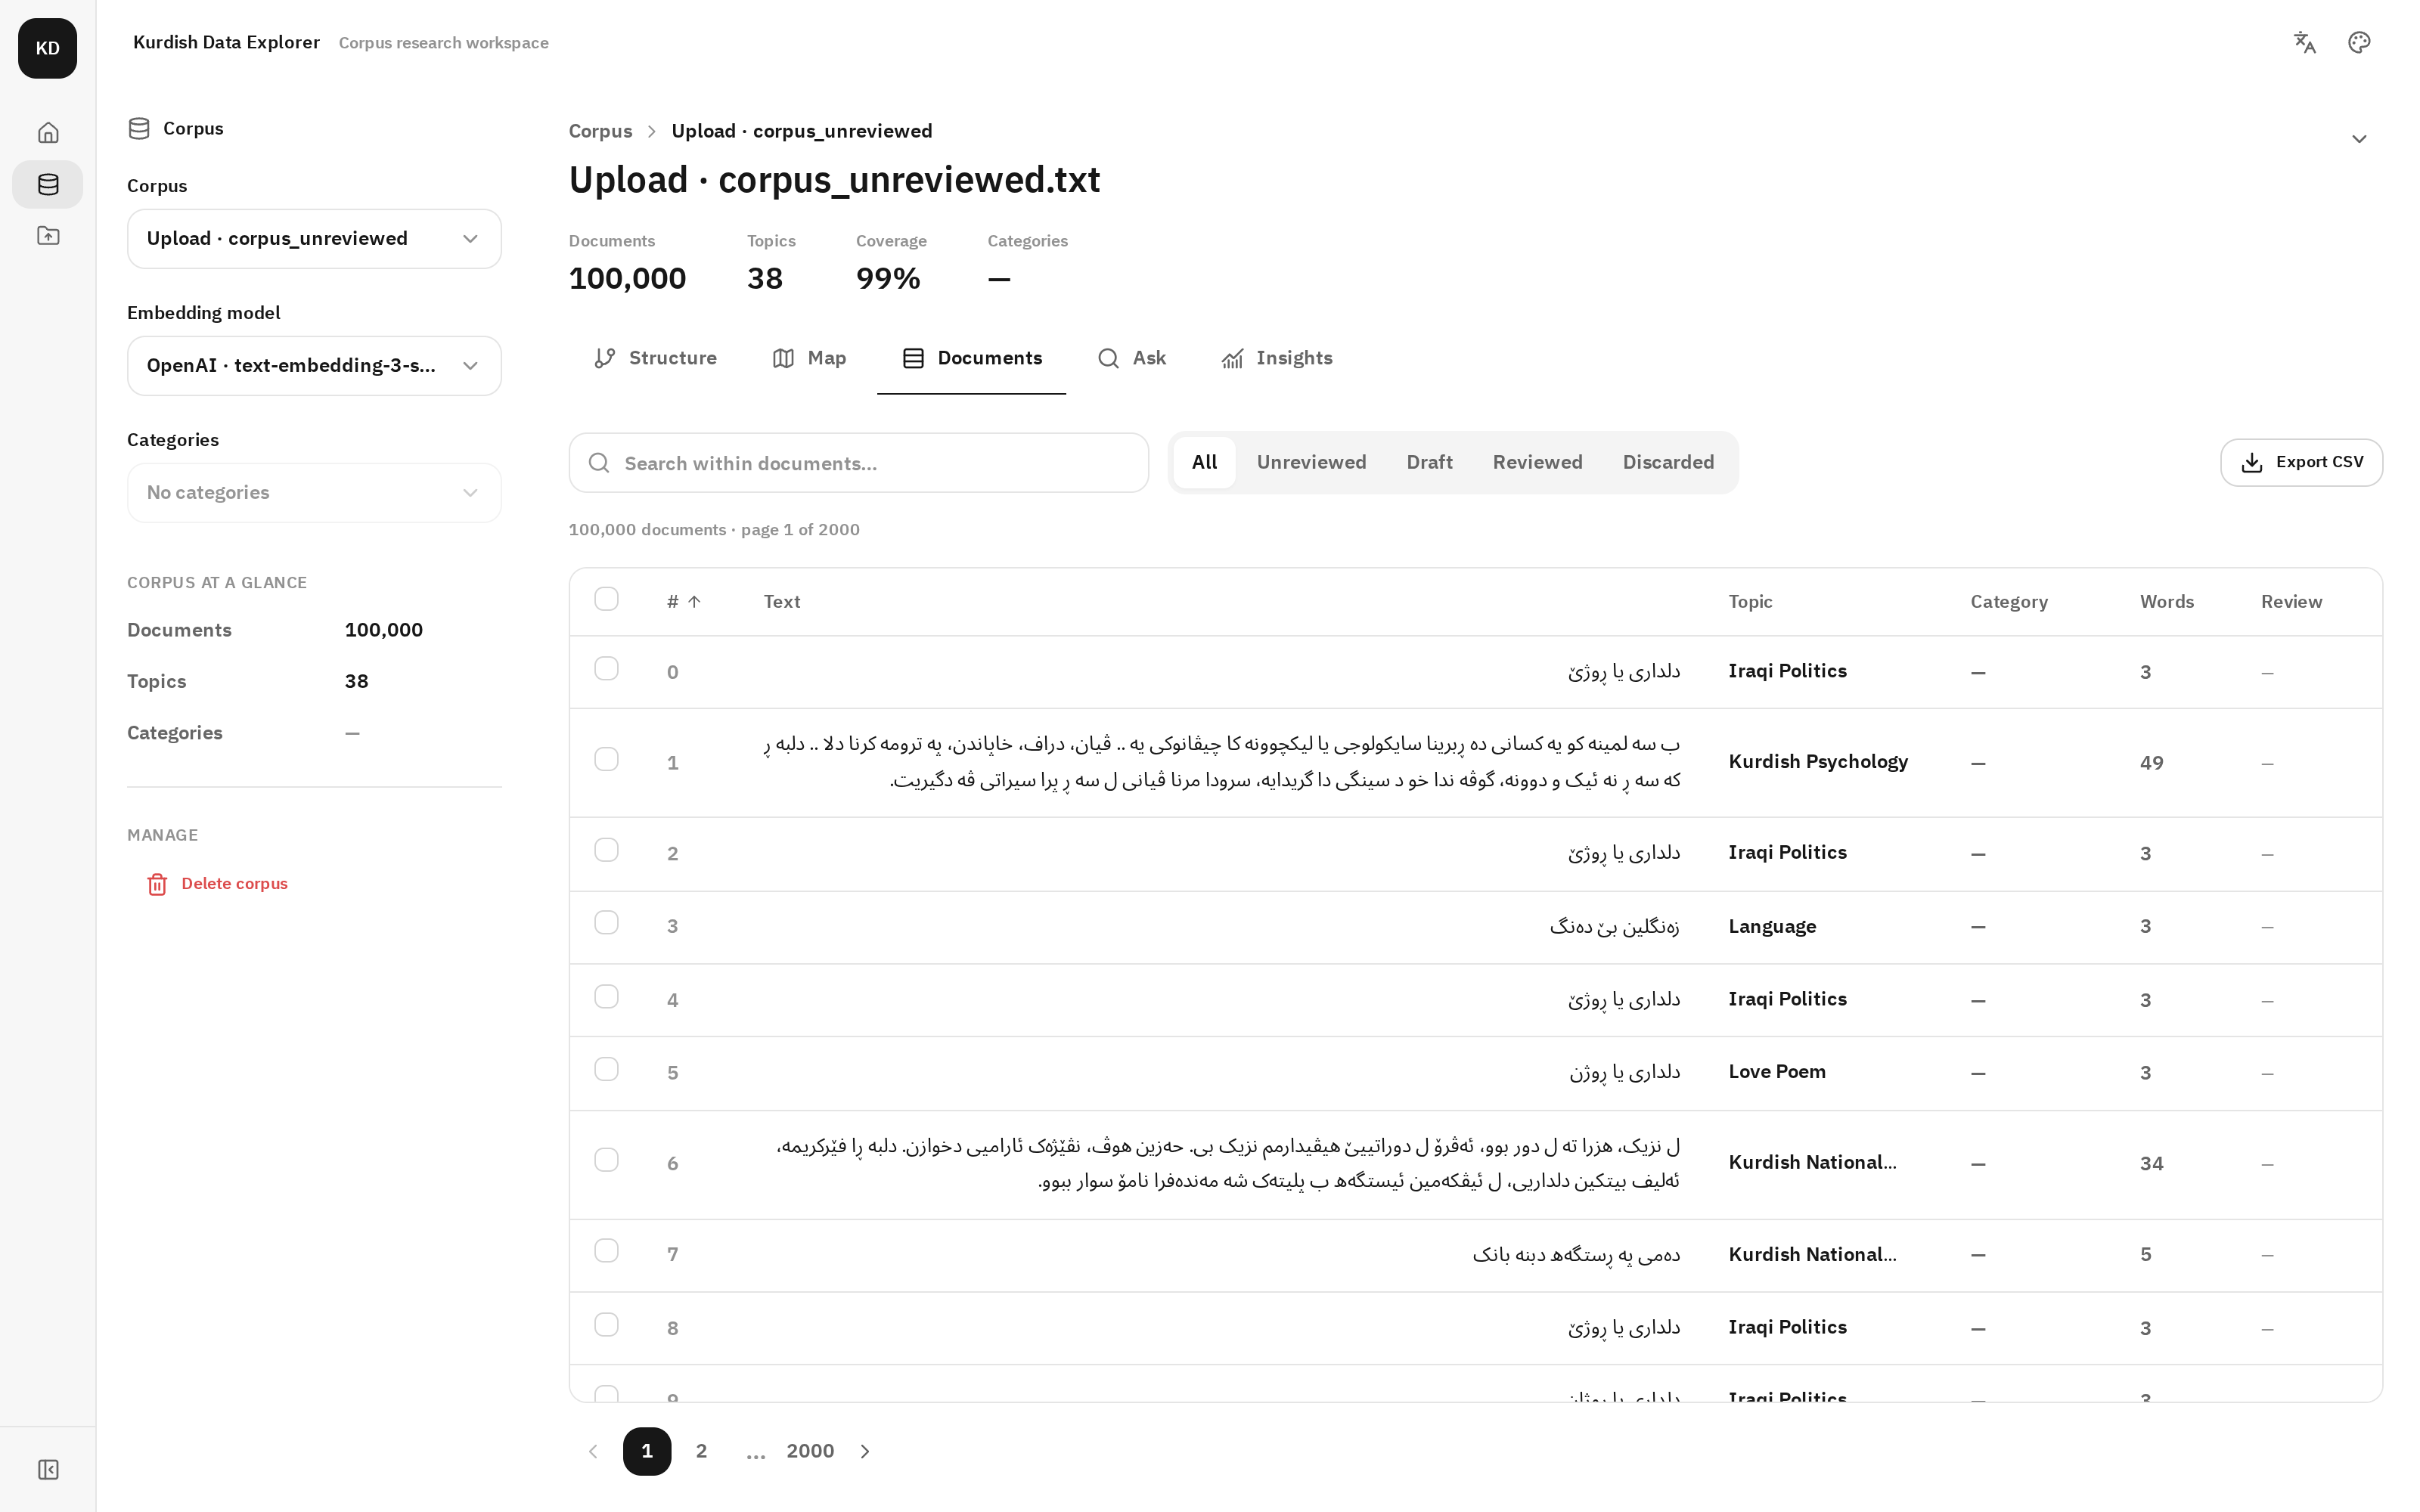
\includegraphics[width=\linewidth]{04-documents-openai.png}
\caption{Documents workspace: searchable table, topic assignments, word counts, and review states.}
\end{figure}

\begin{figure}[htbp]
\centering
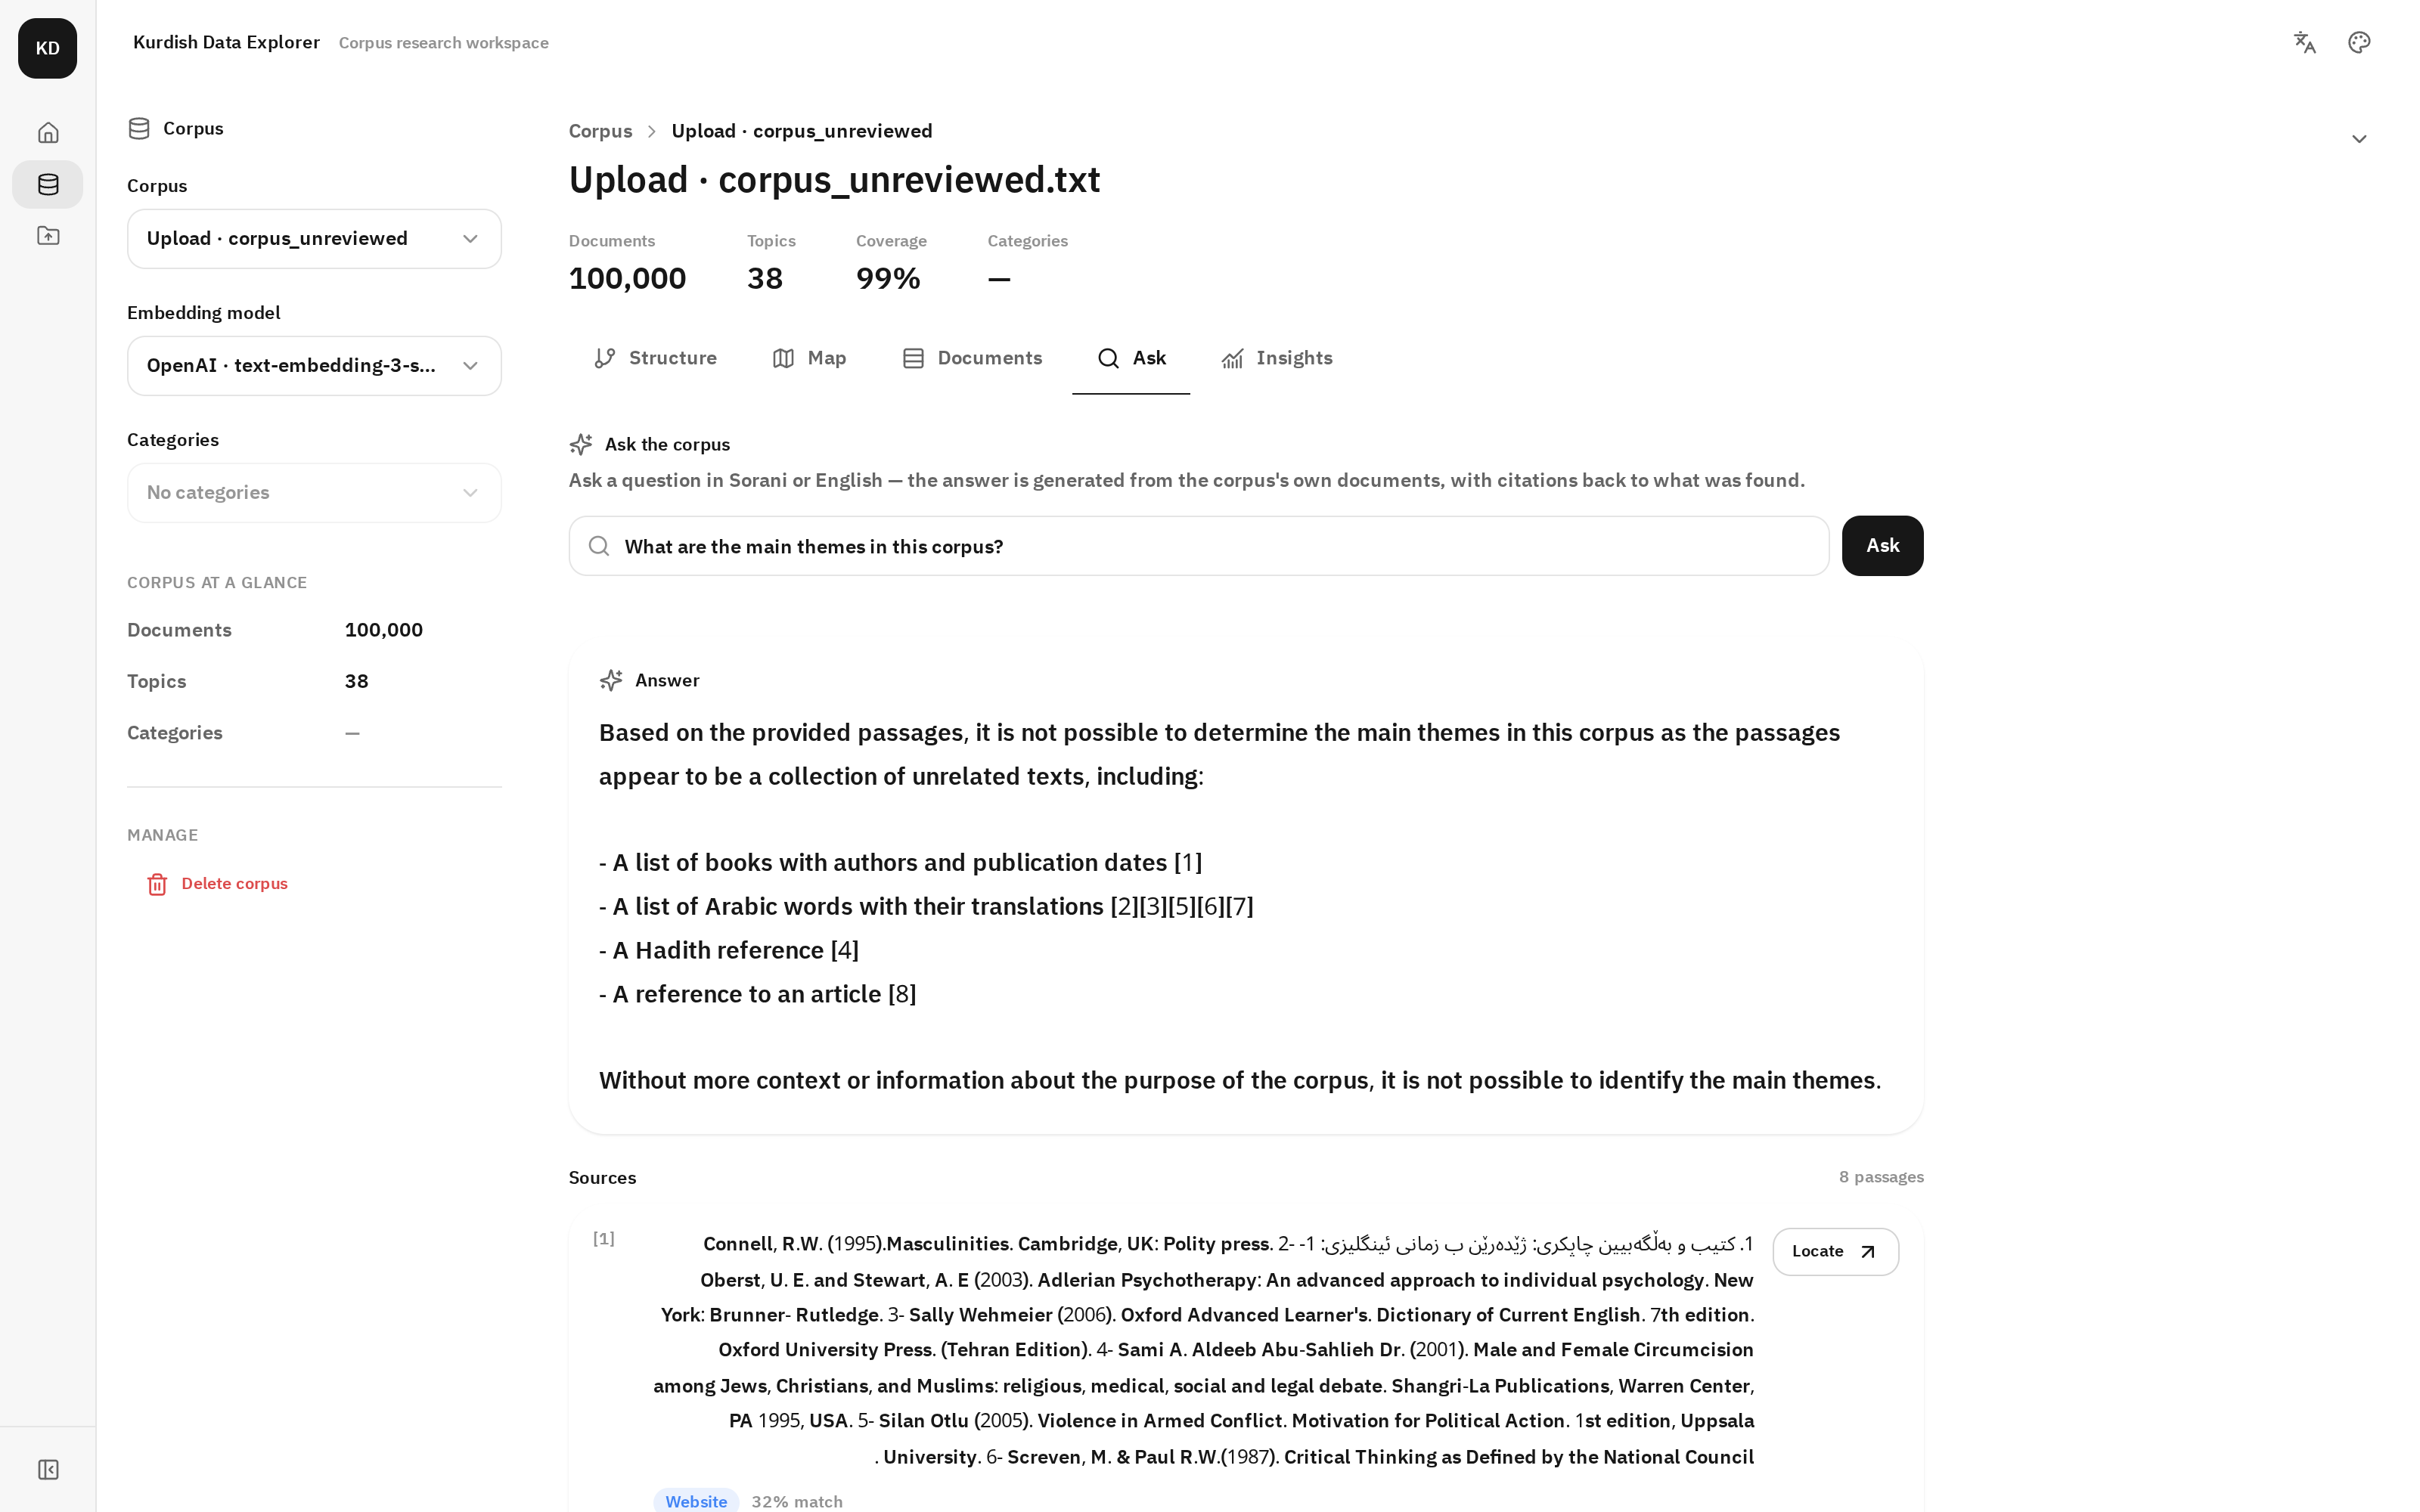
\includegraphics[width=\linewidth]{05-grounded-ask.png}
\caption{Sample input and output: an English question answered from eight retrieved passages. The cautious answer illustrates evidence-bounded RAG behavior.}
\end{figure}

\begin{figure}[htbp]
\centering
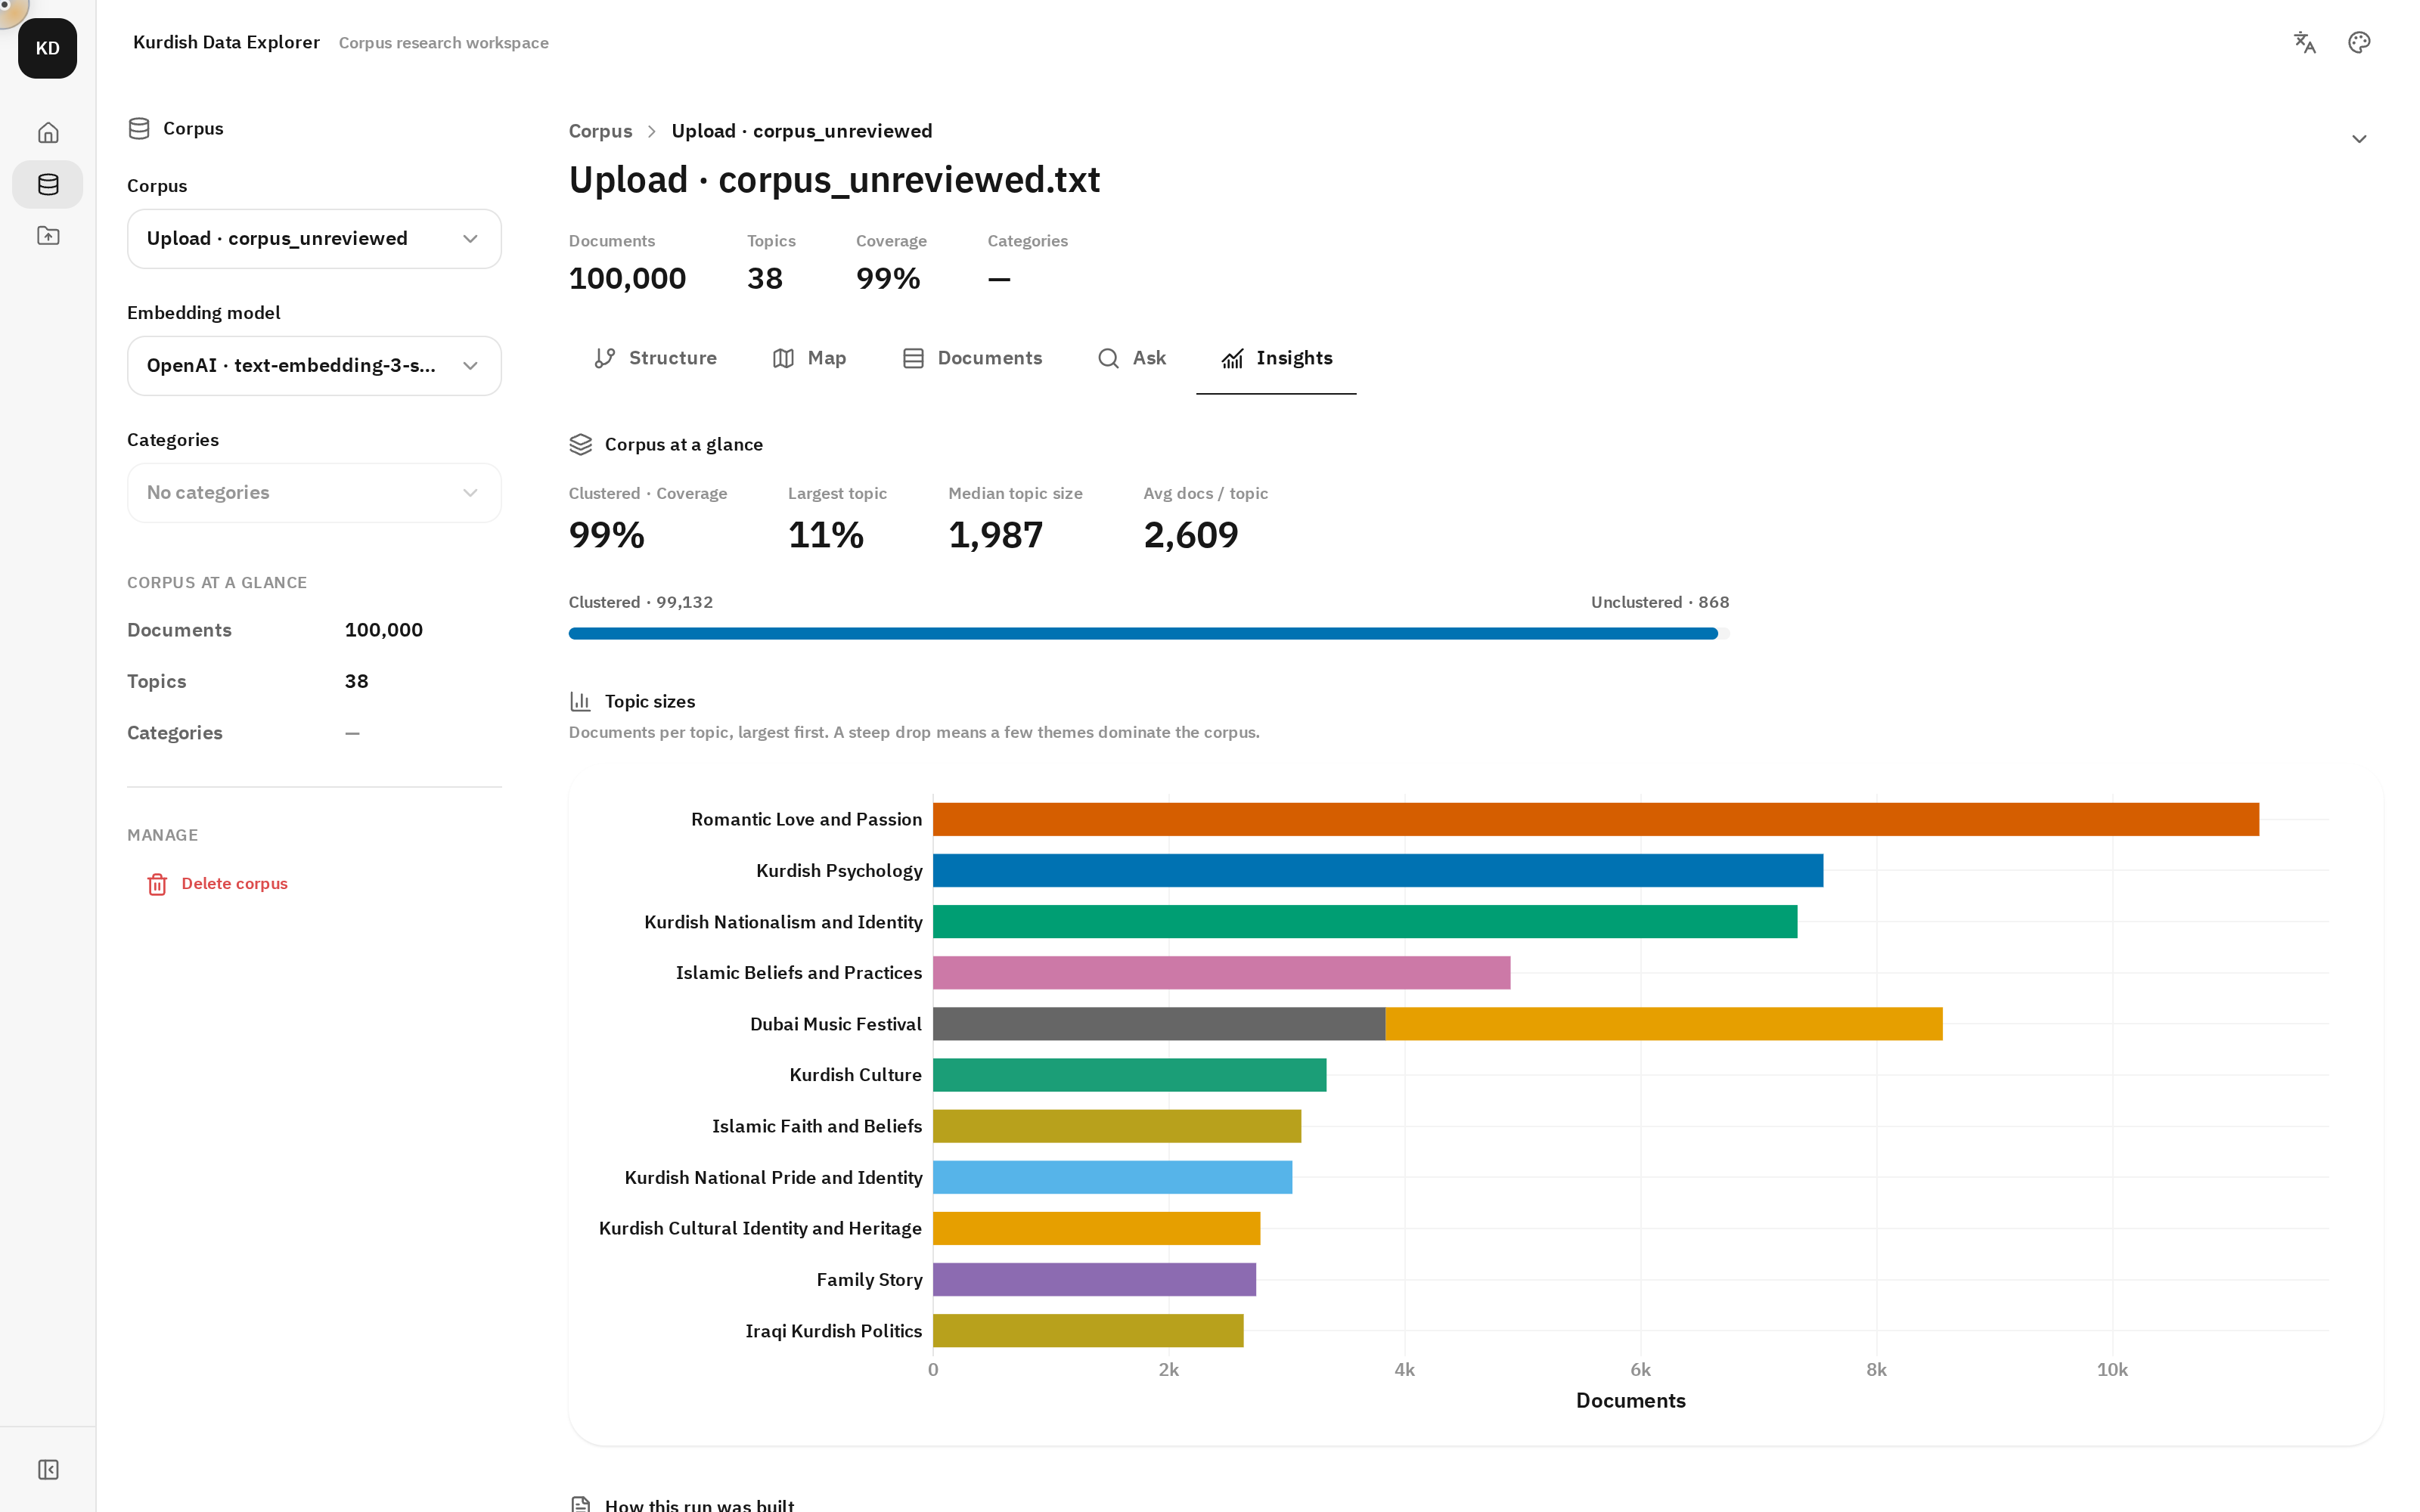
\includegraphics[width=\linewidth]{06-insights-openai.png}
\caption{OpenAI run insights: topic-size distribution and exact run provenance.}
\end{figure}

\begin{figure}[htbp]
\centering
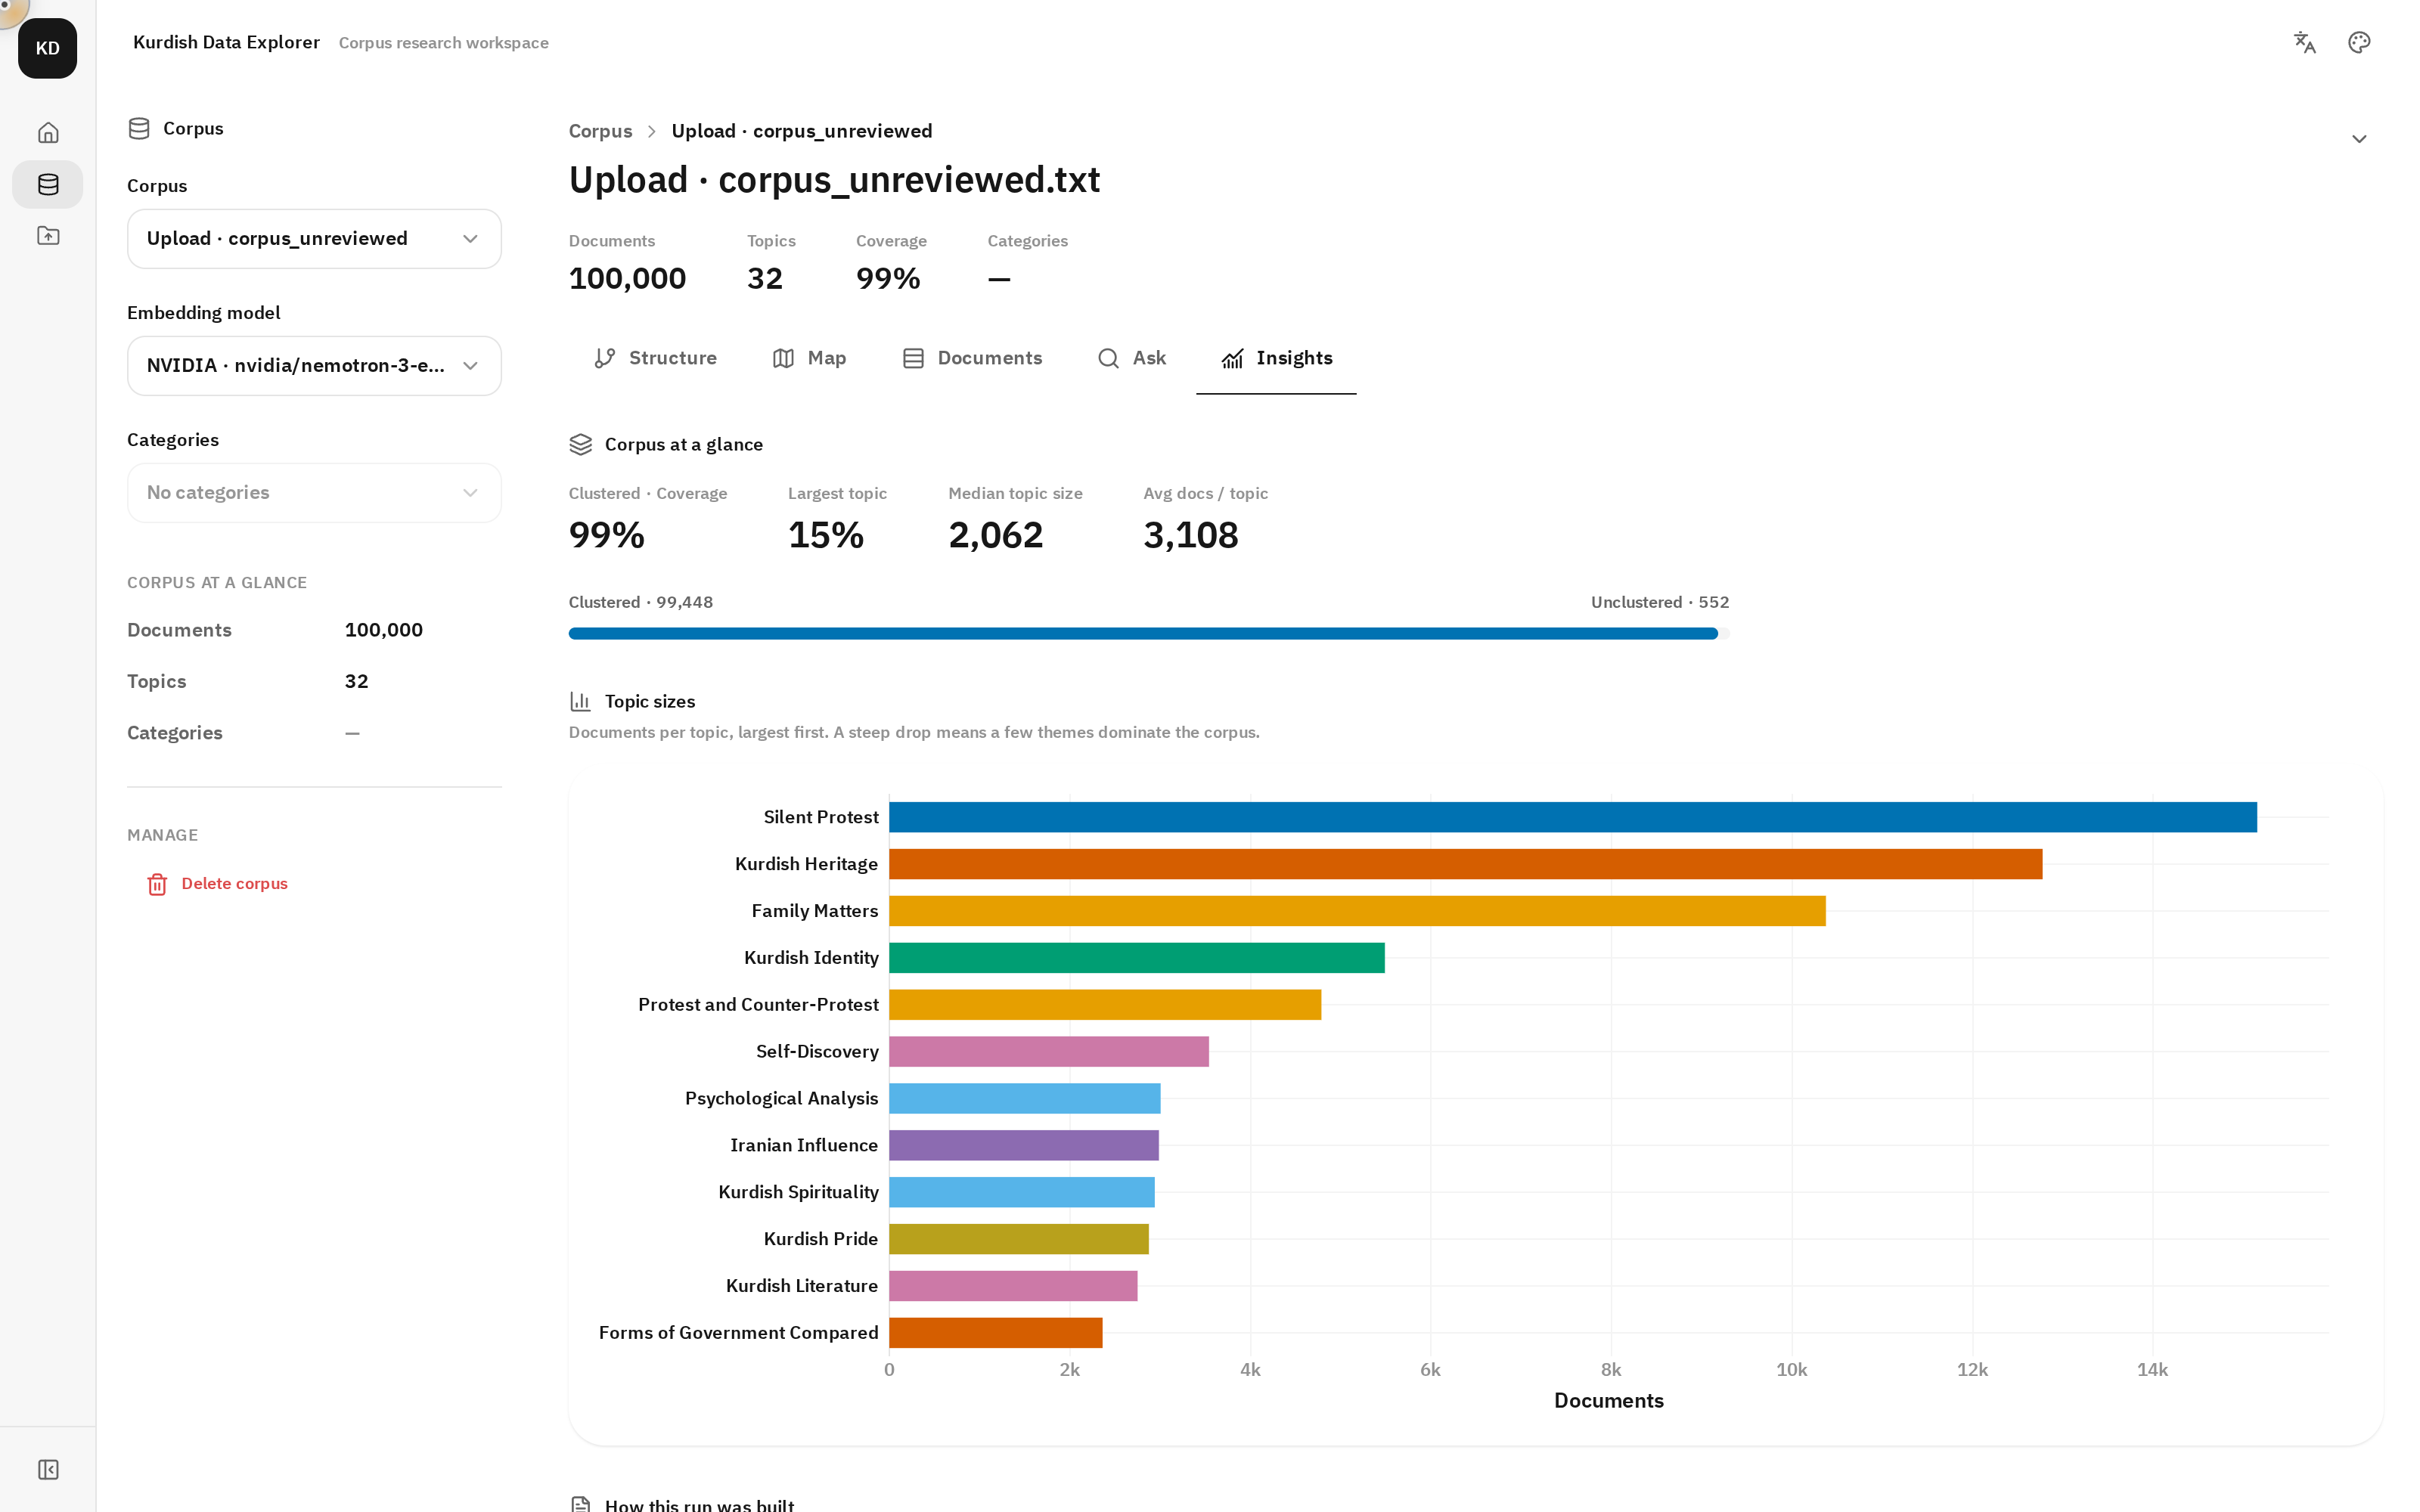
\includegraphics[width=\linewidth]{07-insights-nvidia.png}
\caption{NVIDIA run insights after switching the model selector in the live application.}
\end{figure}

\begin{figure}[htbp]
\centering
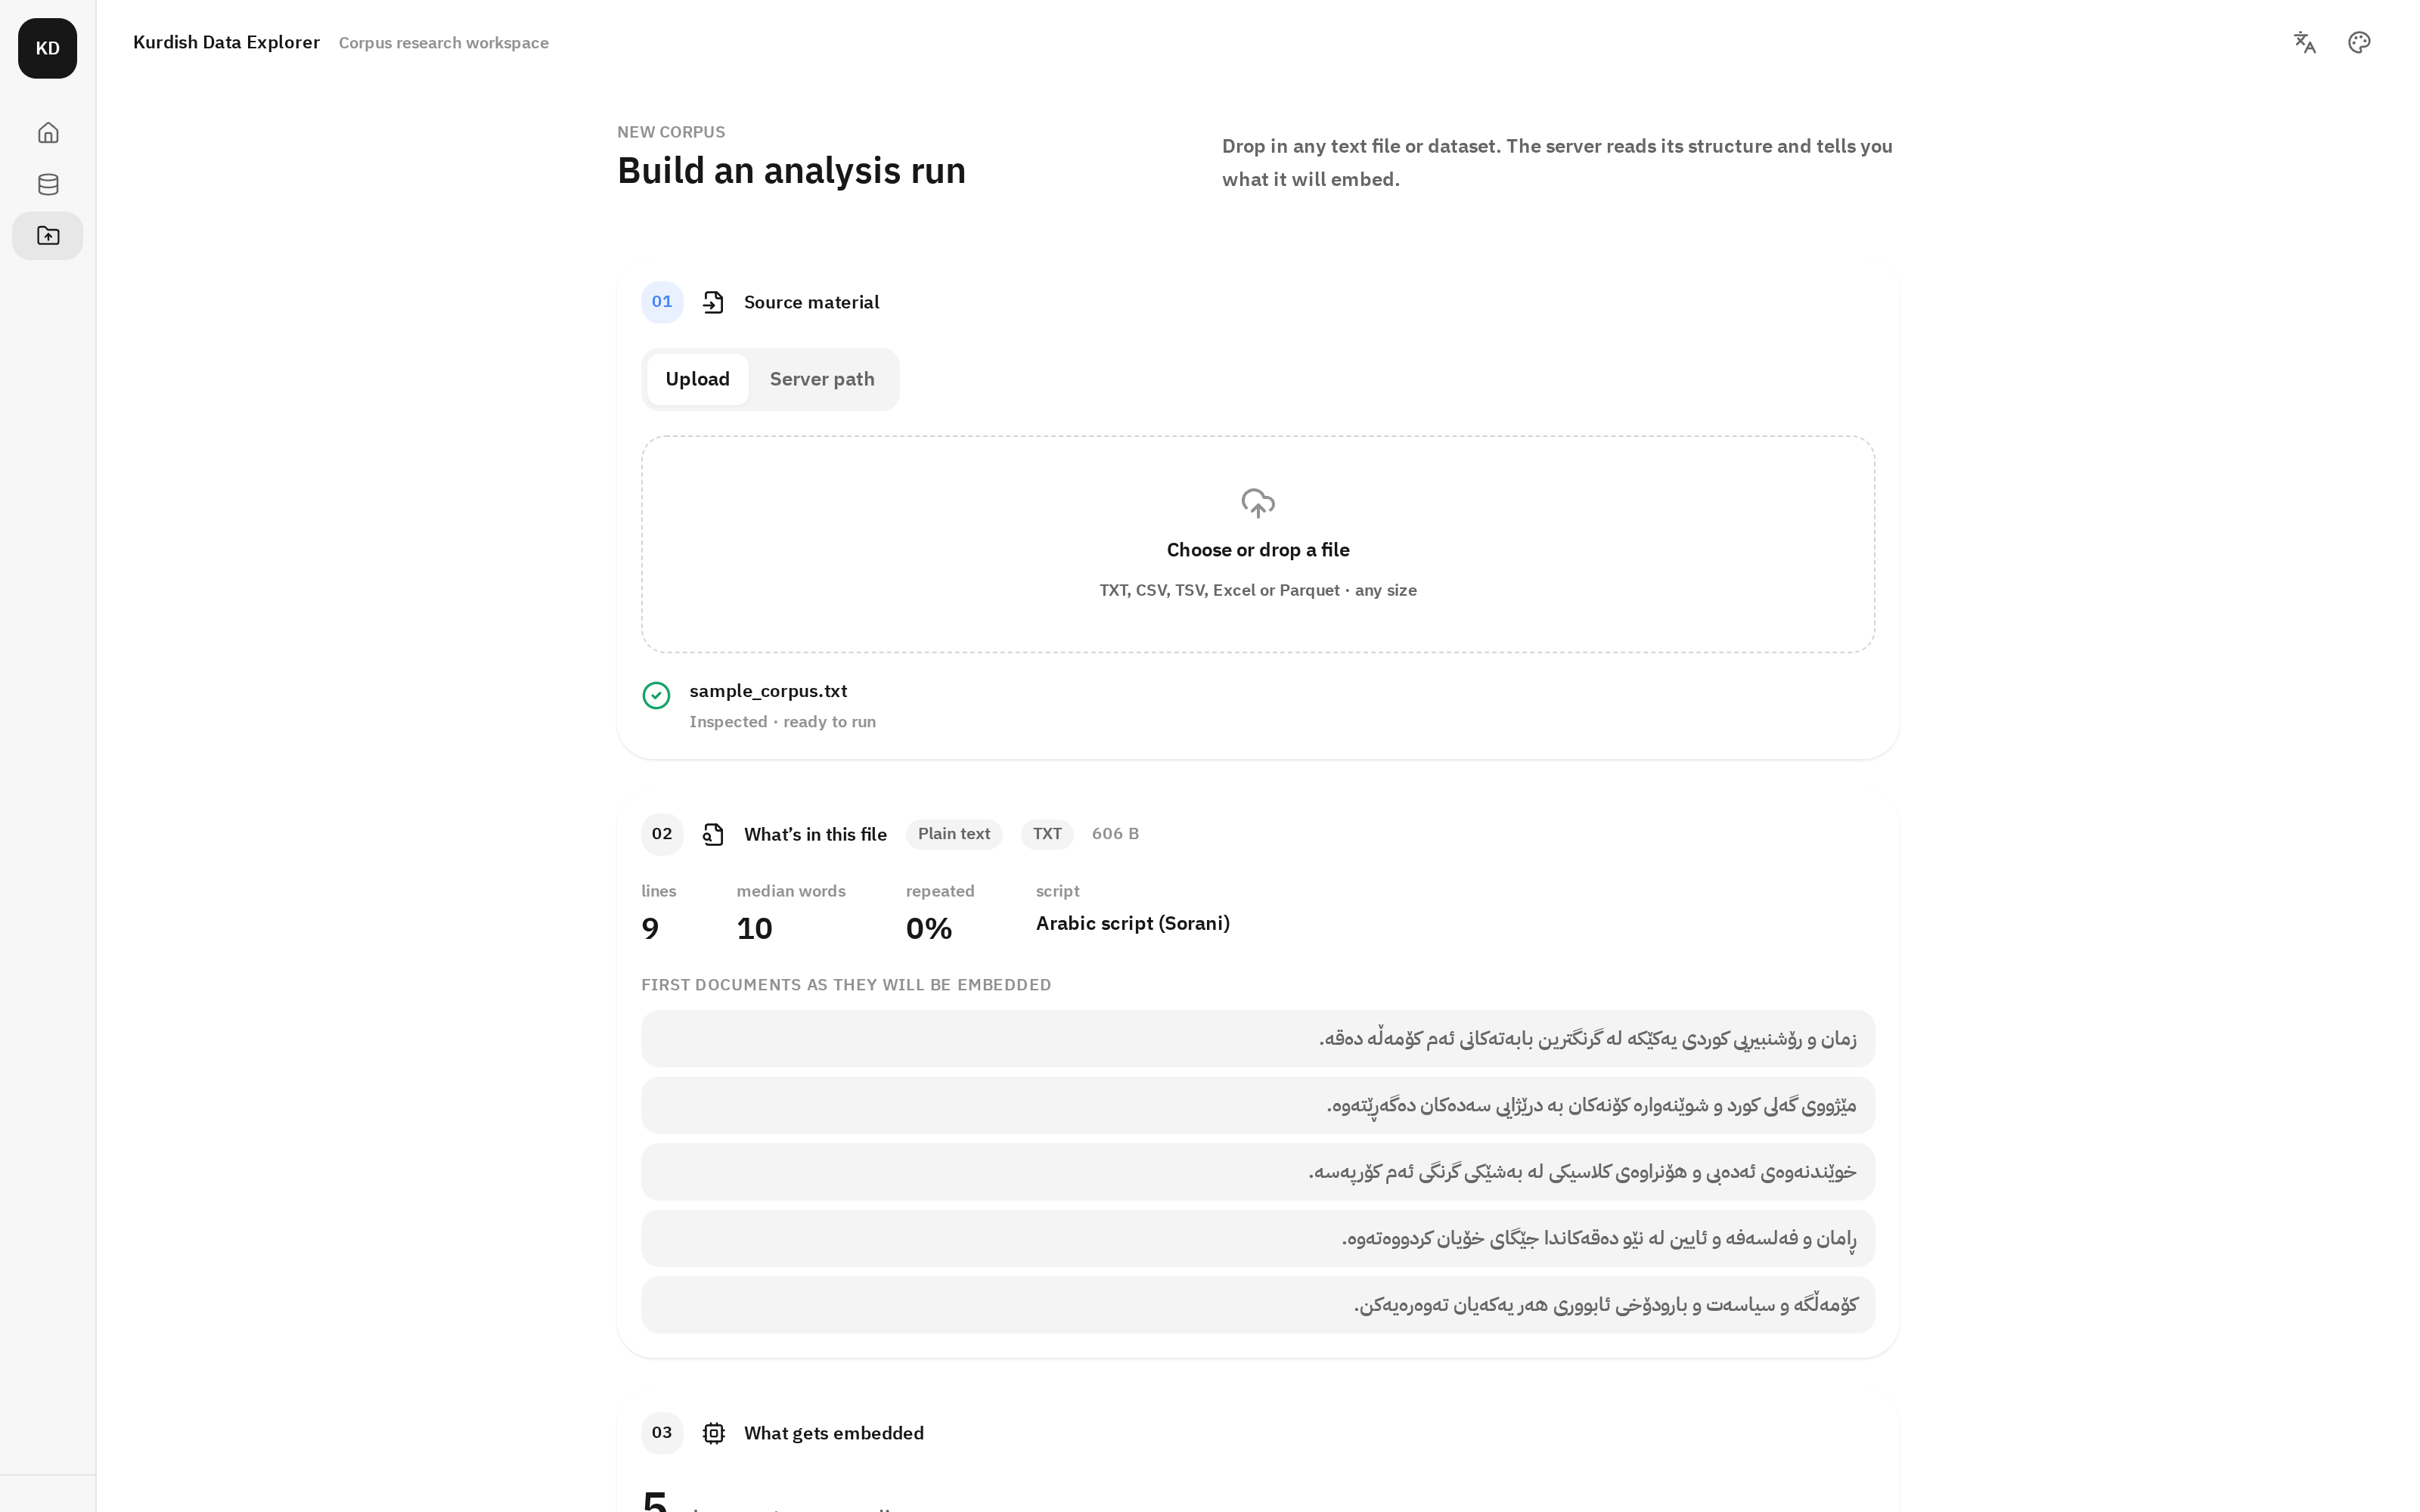
\includegraphics[width=\linewidth]{08-upload-workflow.png}
\caption{Upload workflow for TXT, CSV, TSV, Excel, or Parquet source material.}
\end{figure}

% --------------------------------------------------------------------------
\clearpage
\refstepcounter{section}
\subsection*{Appendix~\thesection: Artifact and Submission Map}
\addcontentsline{toc}{subsection}{Appendix~\thesection: Artifact and Submission Map}

\begin{table}[htbp]
\centering
\caption{Submission requirements and the corresponding project deliverables.}
\small
\rowcolors{2}{RowShade}{white}
\begin{tabularx}{\linewidth}{@{}>{\bfseries}p{38mm}Y@{}}
\rowcolor{Navy}\thc{Requirement} & \thc{Project location or access method}\\
Final report PDF & \sourcecode{reports/final/Kurdish_Data_Explorer_Final_Report.pdf}\\
LaTeX source & \sourcecode{reports/final/main.tex} and \sourcecode{references.bib}\\
Source code & \githubicon\href{https://github.com/SawabS/NLP_KurdishDataExplorer}{github.com/SawabS/NLP\_KurdishDataExplorer}\\
Dataset instructions & \githubicon\href{https://github.com/SawabS/Bahdini_Crawler}{github.com/SawabS/Bahdini\_Crawler}; raw/OCR data are excluded from Git\\
Saved production runs & \sourcecode{artifacts/<source>__<model>/}; production image includes OpenAI and NVIDIA run artifacts\\
Presentation slides & Existing project presentation materials are documented in \sourcecode{wiki/synthesis/project-presentation-overview.md}\\
Deployment & \url{\projecturl}; health endpoint at \url{https://kdx-explorer.fly.dev/api/health}\\
\end{tabularx}
\end{table}

\vfill
\begin{center}
\qrcode[height=38mm]{https://kdx-explorer.fly.dev}\\[3mm]
{\sffamily\bfseries\color{Navy}\large Kurdish Data Explorer}\\
\url{\projecturl}
\end{center}

\end{document}
